\chapter{Harnessing Meta-data}\label{ch:satelliteImages}
% \textcolor{red}{

% \begin{itemize}
%     \item What is the issue of current modelling methodologies?
%     \item \emph{Generalization} and \emph{Complexity}
%     \item How can Generalization be remedied? 
%     \item Obtaining features of propagation scenarios that are generalizable across propagation scenarios
%     \item how can Complexity be remedied?
%     \item 
    
% \end{itemize}}

Any kind of propagation modelling requires data of the propagation scenario. Detailing propagation-specific information requires data and a pipeline, regardless of propagation model. The necessary level of detail is directly related to the accuracy of the channel model. For instance, using principles such as ray-tracing the far-field statistics can be computed with high accuracy, but if and only if, the propagation scenario is described with sufficient detail. Accurate channel models consider a data complexity trade-off. By default, if more data is available, it will offer fewer generalization issues but in return, require a complicated data pipeline for modelling. Less data complexity results in more generalization issues. So, is there a sweet spot where the complexity is low, and the generalization is high? This chapter aims to explore this area and supply an attempt at answering such a question. The requirements for low and high complexity propagation modelling methods is outlined in Chapter \ref{ch:channelmodellingbasics} along with the basics of wireless channel propagation impairments. 


\section{Generalization and Complexity \label{sec:generalization}}



Generalization and complexity is the core issue of path loss prediction. If detailed propagation specific data can be obtained, one can obtain accurate path loss estimates using complex models such as ray-tracing. However, if such data is not available, simpler model using closed-form solutions with simple parameters are useful. It has been shown that both methodologies have their use cases. For instance, simpler path loss models are used for initial link budgets and preliminary studies, while more complex models are used for complex optimization and the research of novel solutions.


Simple path loss models are used in combinations with margins to ensure communication can be established. This however, will result in a margin of optimization and if channel models with higher accuracy could be utilized such a margin could be exploited. This exploitation could result in substantial gains in the overall cost of deployment and further optimization. So why not just use more accurate path loss models? They clearly exist and are well studied. In very simple terms, the data complexity is high and requires substantial efforts. In this chapter, \gls{dl} is applied to path loss estimation. More specifically, a novel \gls{dl} method is developed utilizing geographical images and expert knowledge for improving path loss estimation. Finally, the method is shown to be based on a feasible data complexity with a simplistic data pipeline that require no complex pre-processing procedures, such as required for ray-tracing models (See Section \ref{sec:ray-tracing}).

\subsection{Feature engineering}

Generalization has been a long standing issue for channel models as illustrated in \ref{sec:generalization}. In Machine Learning, the issue of generalization is also well studied and many direct comparisons can be made. It is well known, in the area of Machine Learning, that the features (and the resulting parameters of the model) are directly responsible for the performance on unseen data.  Such is the same in the area of channel models. Thus, it can be said that the performance of channel models are directly related to the input parameters used, or in other words, the features used. A comprehensive study of input parameters (features) and the relation to path loss can be found in \cite{Popoola2019}. 
 
Examples of features used in combination with \gls{nn}: \emph{Longitude, Latitude, Distance, elevation, Altitude, Clutter height, portion through building, height, thickness, transmitting power, street width, building height, building speration, transmitter position, street orientation, base station antenna and rooftop height difference, direct ray, reflected ray from ground, two dominant reflected rays, frequency}

The primary difference between models such as empirical models (See Eq. \ref{eq:uma_nlos_pathloss_max}), and \gls{nn}-based models can be outlined in simple terms. In Machine Learning, the aim is not only to discover the best parameters, e.g. features, but also the best model. Traditional path loss models are the result of significant research and measurement campaigns. Therefor, the path loss models is the result of a curve-fit given parameters that have statistical importance to the path loss. In such cases, the model is known and takes a from that is similar to that of Eq. \ref{eq:pathloss_model} (but with additional terms to account for various attenuation differences).

The features used in \gls{nn}-based models versus traditional path loss models are similar for good reason. Having a complete data-driven approach should ultimately provide with similar answers as research have provided in terms of traditional path loss models. The benefit of working with adaptive models is that statistical knowledge is not necessary and is inferred from obtain observations. For instance, by using adaptive models, features that are not directly related to path loss (or at least by some unknown factor) are used to improve predictive performance. This have benefits and downsides. The benefits are that the performance of the models will improve as more data is obtained. The downside is that the performance can be challenging to evaluate with respect to propagation scenarios inherently different from where measurements have been obtained. With that being said, the end goal of path loss models must be to offer generalization regardless of propagation scenario and the features used. This goal is identical whether a traditional single-slope path loss model is used, or it is the product of training. 

Ultimately \gls{nn} are limited in performance by the engineered features \cite{Alom2019AArchitectures}. Meaning, while the use of traditional \gls{nn} approaches may yield significant improvements to empirical models they are limited by the engineered features. This is not the case for \gls{dl}-based models. such models seek to learn from raw data. In this case we look towards the use of geographical images for improving the estimation of attenuation caused by large-scale parameters.


\section{Use of satellite imagery}

To avoid the need for complicated features, and time-consuming feature engineering aspects, we look towards \gls{dl}. The main principles of \gls{dl} and subsequently \gls{ml} are highlighted in Chapter \ref{ch:mlbasics}. 

A novel methodology for path loss and signal quality parameter approximation using satellite images is proposed in this thesis. The results of the documented methods have resulted in three publications \cite{Thrane2018DriveApproximation, Thrane020ModelAidedDeepLearning, Thrane2020DeepKnowledge}. The main contributions of the publications are introduced in the remainder of this chapter, along with a more in depth discussion and conclusion. The model architecture for providing path loss and received signal quality metrics using satellite images have been under constant evolution. A significant difference in model architecture and complexity can be observed for all proposed methods.  For cohesion, all methods and the resulting performance is outlined in this section. However, all methods share the same essential component, utilizing images for improving signal quality parameter prediction. The evolution of the proposed method can be termed according to the iterations, thus \cite{Thrane2018DriveApproximation} as \emph{version 1 (v1)}, \cite{Thrane020ModelAidedDeepLearning} as \emph{version 2 (v2)} and \cite{Thrane2020DeepKnowledge} as \emph{version 3 (v3)}. 
\begin{itemize}
    \item A summary of \emph{version 1} can be found in Section \ref{sec:summary_version1}. 
    \item A summary of \emph{version 2} can be found in Section \ref{subsec:conclusion_v2}. 
    \item A summary of \emph{version 3} can be found in Section \ref{subsec:conclusion_v3}
    \item Discussion, Conclusion and future outlook can be found in Section \ref{sec:satellite_image_discussion}
\end{itemize}
\noindent
High resolution satellite images of areas are obtainable using such services as the \emph{static API} from Google Maps \cite{GoogleAPI}, or Mapbox API \cite{MapboxWebsite}. The latter is utilized for this work. The idea of predicting path loss from such images stems mainly from the data availability, but also because such images outline the actual details of a propagation environment. The magnitude of details present in high resolution satellite images greatly surpass that of available open-source meta-data used in models such as ray-tracing. In order to formalize the use of satellite images for path loss prediction, several factors and features needs to be considered in order to aid the learning process. Given the empirical knowledge of path loss in outdoor propagation scenarios as presented in Chapter \ref{ch:channelmodellingbasics}, we can hypothesise where such images may offer the most gain. Local variability, is a term describing losses associated with local obstacles in relation to a receiver position for instance, buildings or vegetation. The primary purpose of the satellite images is to assist in determining attenuation related to local variability from imagery that visualize the local area of the receiver. Thus, in order to effectively utilize such images, they must contain information of local variability, e.g. the large-scale fading present in the environment. In order to do so the images must be of high enough resolution such that buildings, vegetation and other structure can clearly be observed.


\subsection{Problem statement}

The function we desire to learn is the received power for a given position in relation to the transmitter. If the reader recall the link-budget from \ref{ch:channelmodellingbasics}. It takes the form
\begin{equation}
    P_{rx} = P_{tx} + G_{tx} + G_{rx} + L_{rx} + L_{tx} + \underbrace{L(x,y)}_{\text{Path loss}}
\end{equation}
The received power is dependent thus on constants, such as transmission power, gains associated with the transmitter and receiver and losses hereof. The mostly unknown constant of the link budget is dependent on the position in the radio environment. Thus the function we desire to learn consists of constants, and a function that is positional dependent.  

The task is to obtain a model that can continuously predict received power given an image and some position location features. In the world of \gls{ml}, such a model is of type \emph{regression} and follows the form:
\begin{equation}\label{eq:dl_model_satellite}
    t_n = y(x_n, \mathbf{w}, \theta) + \epsilon
\end{equation}

Where $y(\cdot)$ is the function we desire to learn given input parameters $x_n$, a set of learned weights $\mathbf{w}$ and some hyper-parameters $\theta$. We define the output of the model $t_n$. Different techniques can be used to learn the function $y(\cdot)$, in this work \gls{dnn} are used due to the use of images. The methodologies associated with vision type models are rooted in \gls{nn}-based models.



We define the a single input to consists of the following

\begin{equation}\label{eq:dnn_inputs}
    x_n = [\text{lat}, \text{lon}, B_{tx}, d_{\text{lat}}, d_{\text{lon}}, d, \mathbf{A}]
\end{equation}

$\text{lat}, \text{lon}$ identify the geographical coordinates of the receiver, $B_{tx}$ is a variable used to identify the transmitter. $ d_{\text{lat}}, d_{\text{lon}} $ denote the distance in latitude and longitude direction respectively. $d$ denote the distance straight as the crow flies. It is important to note that the only engineered features are the distance metrics, as they are derived based on position of the receiver and the transmitter. $\mathbf{A}$ is used to denote the image of the local area around the receiver position. 

In order to be able to capture and process images, principles from computer vision are applied. This is termed \gls{cnn} as described in Section \ref{sec:convolutions} and uses convolution operations to process the properties of images.

This is posed as a supervised learning problem, thus for each system input ($x_n$) a target is required ($t_n$). The LTE-A reference parameter \gls{rsrp} is used as a definite approximation of received power for the transmitting base station. \textcolor{red}{Define RSRP}. Thus $t_n = \text{\gls{rsrp}}$. It should be noted that several targets can be assigned for the same input, as accomplished in \cite{Thrane2018DriveApproximation}, such as \gls{rssi} and \gls{sinr}. The reason for not including these in later research are described in Section \ref{sec:satellite_image_discussion}.

To learn in a supervised fashion, a cost function is required. The sum-of-squares error function between the model output and the observation is used Eq. (\ref{eq:sum-of-squares}). If recalled, minimizing such an error function corresponds to maximize the likelihood function if the targets have noise that is Gaussian distributed. This is also denoted as $\epsilon \sim \mathcal{N}(\mu,\,\sigma^{2})$ from Eq. (\ref{eq:dl_model_satellite}). If the reader can recall from Chapter \ref{ch:channelmodellingbasics}, the distribution of local variability, e.g. large-scale fading can be approximated with a log-normal distribution. We thus assume, that the observations of $t_n$ are under the influence of large-scale fading.

The optimization is complete using principles of gradient descent and back propagation, as detailed in Section \ref{sec:neural_networks}.



\subsection{Images}


\begin{figure}[h]
    \centering
    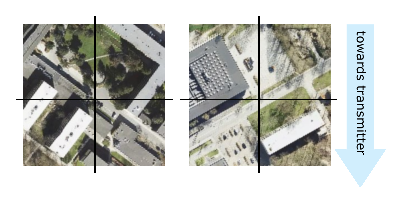
\includegraphics{chapters/part_pathloss/figures/satellite_example.eps}
    \caption{Example of satellite images and the proposed rotation to separate transmitters in same locations.}
    \label{fig:satellite_example}
\end{figure}
A single image of size $256 \times 256 \times 3$ (width, height, RGB color channels) was obtained for each measurement. The area spanned by the images corresponds to roughly $180 m^2$. The reasoning for the image size and the area covered was mainly sparked from the observed level of detail. The images contain a large enough area to display important buildings and vegetation with sufficient detail. When constructing the dataset with the images, two main concerns arose
\begin{enumerate}

    \item Measurements from different transmitters at the same position, how would the images need to differ?
    \item How to embed distance between transmitter and receiver?
\end{enumerate}

The approach for 1) was to rotate according to the transmitter. That way, images are the same area (or same position even) were inherently different. A fixed image size is simplifies the \gls{dl} model greatly, so it was avoided to embed further information into the images. to ensure 2) is addressed, the distance was thus given as a feature along with the positional locators. This ensure the primary objective of the images, is to offer information of geostatistics representing local variablility. An example of such a rotation can be seen in Fig. \ref{fig:satellite_example}.



\section{Signal quality prediction utilizing Satellite images (v1)}\label{sec:initial_v1}
The system documented in \cite{Thrane2018DriveApproximation} explores the use of colourized satellite images and multiple signal quality metrics as output, e.g. \emph{v1}. The inputs are separated into two neural networks and at a later stage combined into a deep output layer. The inputs and outputs can be observed in Fig. \ref{fig:dnn_architecture_drive_test_minimization}. For this work, the approach was to develop a method that can minimize drive testing, as this is an expensive practice as also highlighted in section \ref{sec:drive_testing}.

\begin{figure}
    \centering
    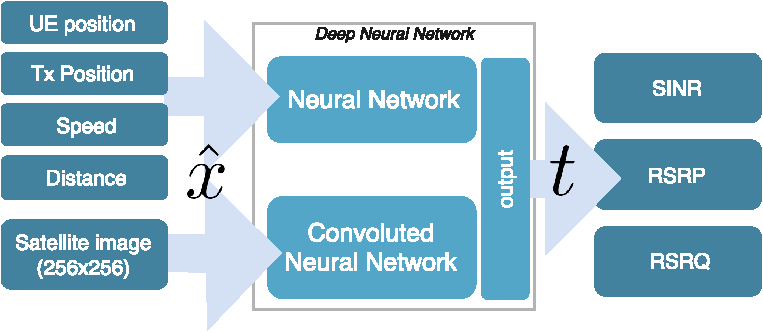
\includegraphics{chapters/part_pathloss/drive_test_minimzation_paper/input_output_figure.pdf}
    \caption{Model architecture used in \cite{Thrane2018DriveApproximation} with a multiple of outputs. Two neural networks are used and concatenated at the output layers.}
    \label{fig:dnn_architecture_drive_test_minimization}
\end{figure}

The size of the layers for both the convolutional neural network and the regular neural network can be seen in Table. \ref{tab:dnn_architecture_drive_test_minimization}

\begin{table}[ht]
  \centering
  \caption{Architecture and layer size of the model used in \cite{Thrane2018DriveApproximation}.}
  \label{tab:dnn_architecture_drive_test_minimization}
  \begin{tabular}{l|l|l}
                & NN settings     & CNN settings      \\ \hline
  Layer size & $[40, 40]$      & $[32, 16, 16, 8]$ \\
  Dropout       & $0.3$           & $0.1$             \\
  Activation    & \textit{ReLU} & \textit{ReLU}  
\end{tabular}
\end{table}

The only regularization added to the model weights were done using dropout layers. The use of dropout layers further enabled so-called \emph{Bayesian approximation} through Monte-Carlo sampling of the layers. The principles are explained in Section \ref{sec:neural_networks}. 

The drive tests detailed in Appendix \ref{app:drive_test_study_2017} compromised the foundation for the data set used for training. The measurements were split into more defined routes as to \emph{emulate} the process of a drive-test and thus limit the available amount of training examples. A total of $39000$ input and target pairs constructed the data set. Of the $\sim 39000$, $\sim 9000$ compromised the test set, as also shown in blue in Fig. \ref{fig:drive_test_routes_split}. Two specified routes, \texttt{Route 1} and \texttt{Route 2}, compose the testing set. Colourized images were used as input to the Deep Learning model. The images were downloaded from Mapbox API \cite{MapboxWebsite}. The colourized images were rotated according to the transmitter to distinguish images at the same position but from different transmitters.

\begin{figure}
    \centering
    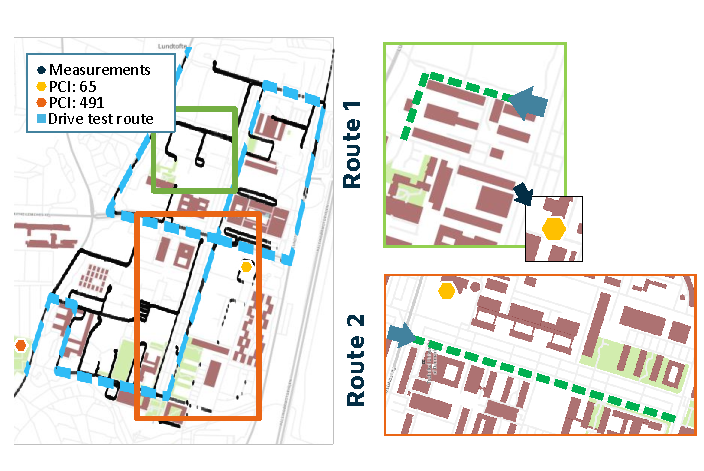
\includegraphics{chapters/part_pathloss/drive_test_minimzation_paper/route_drawing.pdf}
    \caption{The majority of roads at DTU campus area were covered during drive testing. The training was isolated to the main roads of campus, while two specific routes were isolated for testing and evaluation, \texttt{Route 1} and \texttt{Route 2}.}
    \label{fig:drive_test_routes_split}
\end{figure}

The implementation and training of the model was done with open-source libraries \emph{Keras} \cite{chollet2015keras} with \emph{TensorFlow} \cite{tensorflow2015-whitepaper}. The training was accelerated with GPU and mini-batch training. The batch size was heavily limited by the RAM available on the GPU device and was thus limited to $5$. 


\subsection{Results}
\begin{marginfigure}
    \centering
    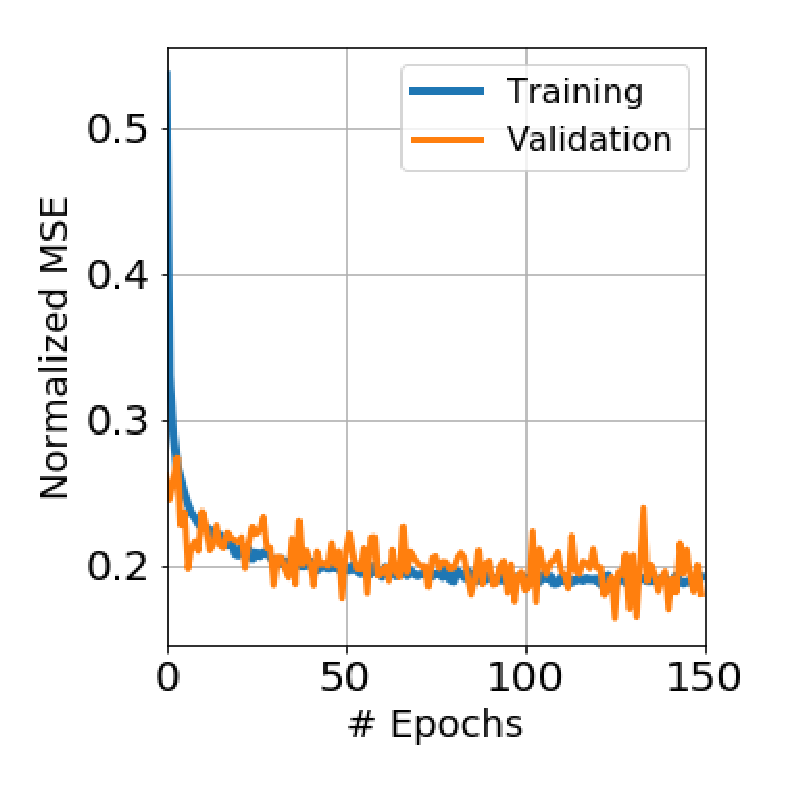
\includegraphics{chapters/part_pathloss/drive_test_minimzation_paper/training_val_test_5ab7fb562d60543b24f857af.eps}
    \caption{Training and validation error for the training of the model.}
    \label{fig:training_val_error}
\end{marginfigure}

The \gls{rmse} error for both rest routes can be observed in Table \ref{tab:rmse_error_v1} for all output metrics. The sampled standard deviation $\sigma$ using the Bayesian approximation method is also presented. The standard deviation can also be presented in terms of a confidence interval, as visualized in Fig. \ref{fig:route_1_v1} (RSRQ as a function of measurement) and \ref{fig:route_2_v1} (RSRP as a function of measurement) along with the prediction (the mean $\mu$) for both rest routes. The measurements are sorted sequentially so the route progression can be studied. This allows for the evaluation of the obstacles during the measurement sequence. For instance, a large obstacle (building) is observed in the radio environment and can be identified by the prediction of the model. 

The \gls{rsrp}, as a function of measurements for route 2, is shown in Fig. \ref{fig:route_2_v1}. It can be seen that a significant decrease in \gls{rsrp} is observed for both predictions and measurements. The decrease in \gls{rsrp} is due to the sequence of measurements. The sequence is increased separation between the transmitter and the receiver, i.e. the vehicle moving away from the \gls{enb}. The trained model captures this and provide sufficient predictions of \gls{rsrp} with an added confidence interval. Most of the measurements are within the $95\%$ confidence interval, which illustrates the usefulness of the Bayesian approximation. 

The training and validation error is shown in Fig. \ref{fig:training_val_error}. The final test error performance of the system (in terms of normalized MSE) was observed to be $\mathbf{0.37}$ MSE. 

\def\arraystretch{1.5}
\begin{table}[]
\centering
\begin{tabular}{@{}lll@{}}
\toprule
\textbf{Parameter} & RMSE   & $\pm \sigma$ \\ \midrule
SINR               & $5.2$ dB & $4.1$ dB       \\
RSRP               & $7.7$ dB & $5.9$ dB       \\
RSRQ               & $3.1$ dB & $2.2$ dB       \\ \bottomrule
\end{tabular}
\caption{\gls{rmse} for both rest routes with the sampled $\sigma$ }\label{tab:rmse_error_v1}
\end{table}



\begin{figure}
    \centering
    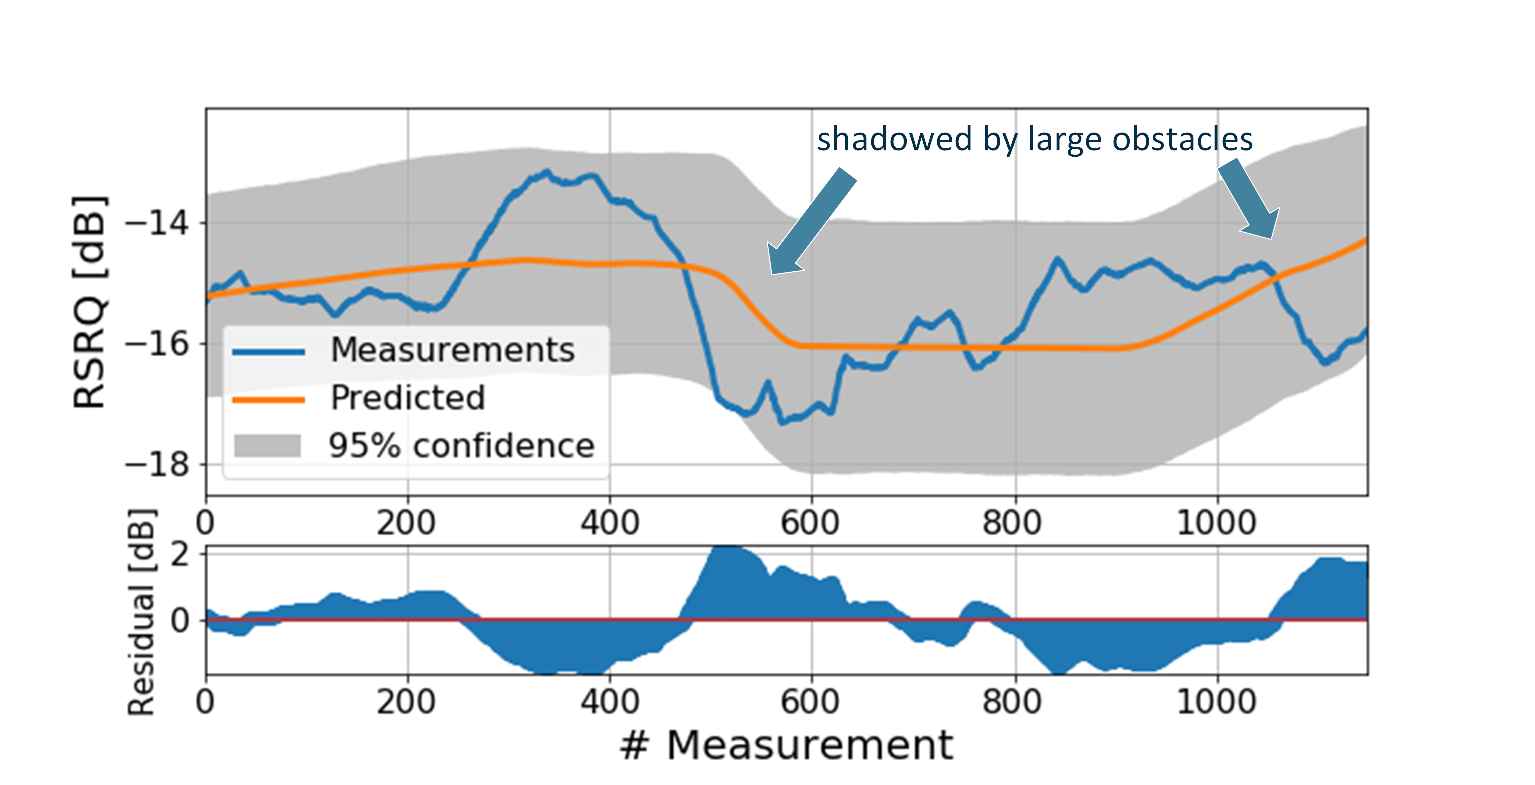
\includegraphics{chapters/part_pathloss/drive_test_minimzation_paper/route_1_predictions_5ab708662d60543b24f857a1_annotated.eps}
    \caption{Prediction of \texttt{route 1} \gls{rsrq} with added $95\%$ confidence interval.}
    \label{fig:route_1_v1}
\end{figure}


\begin{figure}
    \centering
    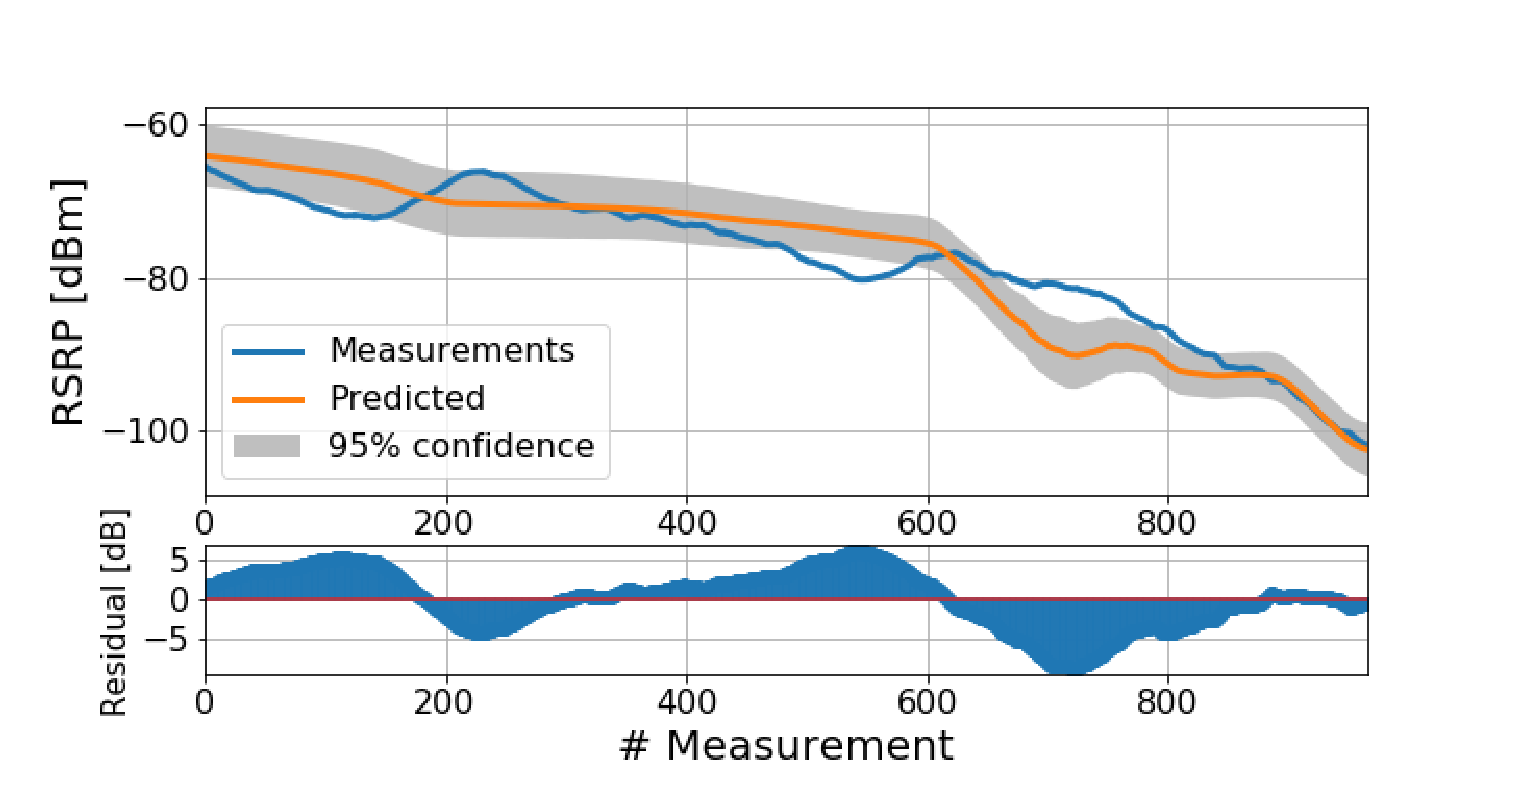
\includegraphics{chapters/part_pathloss/drive_test_minimzation_paper/route_2_predictions_5ab708662d60543b24f857a1.eps}
    \caption{Prediction of \texttt{route 2} \gls{rsrp} with added $95\%$ confidence interval.}
    \label{fig:route_2_v1}
\end{figure}

\subsection{Discussion and Conclusion}
It has been shown that the trained model is capable of providing accurate predictions in unseen areas using limited training data. This was evaluated using two independent routes for testing, e.g. \texttt{route 1} and \texttt{route 2}. From the prediction results of \texttt{route 1}, it was observed that the model is capable of achieving some insight into the local variability. However, it is unknown if the images or sufficient information causes this insight through distance features. It does indicate that the satellite images are useful; however, it requires further studies. 
For \texttt{route 2}, the model is observed to be capable of providing a decrease in \gls{rsrp}, which is primarily related to transmitter and receiver separation distance. 

In terms of model generalization, some issues exist. This is highlighted by the gap between training/validation and test error; thus, further model regularization can improve the overall prediction accuracy of the system. In summary, the \emph{version 1} of utilizing satellite images provided the following conclusion

\begin{itemize}
    \item The model is capable of predicting a drop in \gls{rsrq} explained by the shadowing of a large building.
    \item The model is capable of predicting an accurate decrease in \gls{rsrp} as a function of transmitter-receiver antenna separation.
    \item The gap between training and test error highlights generalization issues
\end{itemize}

It is thus of interest to explore 1) the specific prediction improvements caused by images and 2) the generalization of the model (and techniques hereof).

\section{Generalization issues}\label{sec:summary_version1}
The method has some shortcomings, especially related to generalization. The gap between the test and training set is seen as being significant. However, and possibly most interesting, the documented work introduces the novel idea of introducing automatized meta-data extraction for use in path loss estimation.
As recalled by section \ref{sec:generalization}, \glspl{nn} are capable of providing a satisfactory regression solution to path loss prediction. It is possible and likely that the majority of the accurate path loss predictions are directly related to the primary feature \emph{distance}. The results show that some large-scale fading impairments can be predicted; however, it is unknown if this is due to image-related features. Further studies were deemed a necessity. Specifically, a benchmarking study against traditional path loss prediction methodologies would identify and quantify both the shortcomings and benefits of the documented method. Additionally, it is of interest to study the specific performance gain offered by the inclusion of images. Such a study was completed and published in \cite{Thrane020ModelAidedDeepLearning}.  

\section{Embedding expert knowledge (v2)}\label{sec:expert_v2}
The architecture of the method was completely revised for the second study to ensure the possibility of validating and studying two particular aspects that are of interest:

\begin{itemize}
    \item Generalization improvements by aided learning (expert knowledge)
    \item Performance improvements by images
\end{itemize}

Obtaining generalization in any \gls{ml}-type solutions remains the primary objective of any engineered \gls{ml} solution. Recently, papers introducing model-aided learning have gained popularity due to the achieved generalization properties and the overall simplification in the learning process. It is argued that scientists over the recent decades have constructed quite good models for the reality we live in, and such models should be utilized in \gls{ml} processes. 

What sparked the idea and interest was the work detailed in \cite{Zheng2016}, where a robot is tasked with throwing and catching objects. To throw and catch objects accurately, a predictive model is necessary. The authors show that by utilizing a basic ballistic model for predicting the trajectory in combination with a \gls{ml} system, significant performance gains can be achieved. More specifically, considerable accuracy improvements could be gained by introducing a simple model into the learning process. Even though the model is not accurate, it assisted the learning process to learn the unknown factors associated with the overall throwing system, for instance, the complexity added by the friction of the mechanical joints in the robot etc. This approach reduced the whole learning task from learning the entirety of the system, including the ballistic model, to only learn a correction of the theoretical ballistic model.

Aiding the \gls{ml} models with expert knowledge have been shown to be useful for path loss estimation in \cite{Cavalcanti2017} while expert knowledge for utilization in wireless systems has been hailed as a necessity for future \gls{ml}-based and \gls{dl}-based solutions \cite{Zappone2019}.

Given the recent results of \cite{Thrane2019ComparisonGHz} also seen in section \ref{sec:comparison_ghz_paper}, simple empirical path loss models were evaluated to be valuable. The second version was thus the integration of simple empirical models into the path loss prediction to improve the shortcomings identified in \emph{version 1}. 

\begin{figure*}
    \centering
    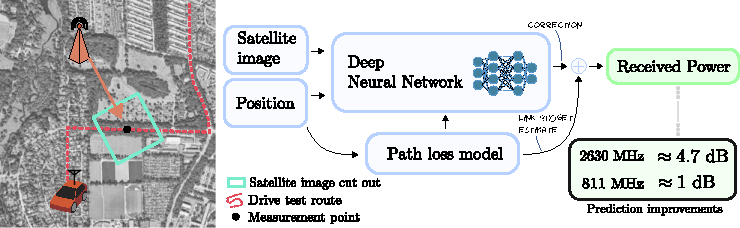
\includegraphics{chapters/part_pathloss/model_aided_paper/version2_approach_figure.pdf}
    \caption{The improved approach introduces expert knowledge for improving training stability and testing accuracy.}
    \label{fig:my_label}
\end{figure*}

\subsection{Model architecture}
The model definition was changed and simplified to adjust to isolated experiments. The previous model architecture provided several output metrics of signal quality, in order to determine the performance increase of the model approach this was isolated to a single output parameter, namely \gls{rsrp}. I.e. we define the model as:

\begin{equation}\label{eq:model}
    y(x_n, \mathbf{w}, \bm{\theta}) = \underbrace{z([x_n, L(d)], \mathbf{w}, \bm{\theta})}_{Correction} + L(d)
\end{equation}

Where $z(\cdot)$ is the model of the \gls{dnn}. The $L(d)$ term is an integrated path loss model and provides an estimated link budget. The link budget is estimated as:

\begin{equation}\label{eq:path_loss_model_linkbudget}
L(d) = PL(d) + G_{tx} + L
\end{equation}

Where $PL(d)$ is the \uma{A} path loss model as detailed in Chapter \ref{ch:channelmodellingbasics}. $G_{tx}$ is the estimated transmission power and related gains (constant). We define $L$ as additional losses, such as cable loss and antenna attenuation (constant). 

The defined model is still formalized concerning regression, e.g. Eq. (\ref{eq:dl_model_satellite}) is still the case, however $t_n = RSRP$ and not a vector including such output metrics of \gls{rsrq} etc. The path loss model is integrated into the supervised learning process, as shown in Fig. \ref{fig:combined_model_approach}. The task of the \gls{dnn} is no longer to learn and approximate the received power by itself, it is aided by expert knowledge: a simplified path loss model. We term the output of the \gls{dnn} a \emph{correction}.


\begin{figure}
    \centering
    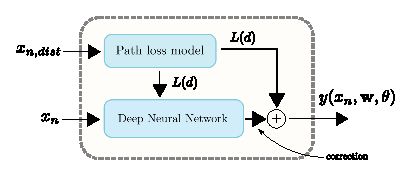
\includegraphics[width=\textwidth]{chapters/part_pathloss/model_aided_paper/combined_model_approach.eps}
    \caption{Combining a path loss model and a \gls{dnn} for estimating \gls{rsrp}.}
    \label{fig:combined_model_approach}
\end{figure}

 $x_{n,dist}$ defines the 3D distance for each measurement point, which, is provided as a feature to the \gls{dnn}. The list of features is the same as presented in Eq. (\ref{eq:dnn_inputs}) with one exception. The estimated link budget is added to the list and is further visualized in Fig. \ref{fig:satellite_model_setup_v2}.
 
The \gls{dnn}, as seen in Fig. \ref{fig:satellite_model_setup_v2} utilize two fully-connected neural networks, and a convolutional neural network. The \gls{nn} termed \texttt{NN} is tasked with managing the engineered features, while the \gls{cnn} is tasked with processing the satellite images. The output of both \gls{nn} are added and combined into a \gls{nn} termed \texttt{NN2}, tasked with processing the information provided by the engineered features and the satellite images resulting in a single output metric. The size of the layers can be seen in Table \ref{tab:cnn_structure} and \ref{tab:nn_structure}.

\begin{figure}
    \centering
    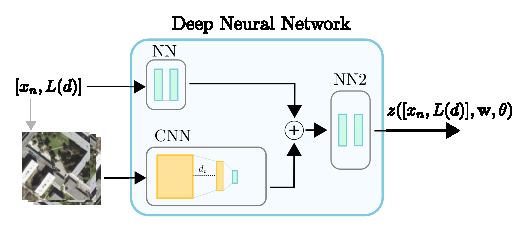
\includegraphics{chapters/part_pathloss/model_aided_paper/setup_model.eps}
    \caption{The Deep Neural Network consists of a convolutional neural network (\emph{CNN}) and two fully connected neural networks, \emph{NN} and \emph{NN2}.}
    \label{fig:satellite_model_setup_v2}
\end{figure}

\subsection{Training}\label{sec:training_v2}
The training of the model was accomplished using Pytorch \cite{Paszke2017AutomaticPyTorch}. The training makes use of backpropagation and the minimization of \gls{mse} loss as described in chapter \ref{ch:mlbasics}. Additionally, the findings of \emph{system v1} highlight the requirement for further generalization techniques. Data augmentation of the images is a common practice to improve dataset size and reduce overfitting during training \cite{Shorten2019ALearning}. The purpose is to feed the algorithm slightly different versions of the same image as to explore the generalization of the method. This was achieved by using a \emph{random  affine  transformation} that shears and rotate the image random but keeps the center of the image invariant. Examples of the data augmentation can be seen in Fig. \ref{fig:data_augmentation}. The transformation utilizes a random rotation angle of $\pm 20$ degrees with $\pm 10$ degrees of shear. The augmentation if applied to the original images for every observation, e.g. for every training iteration. In other words, the original images supplied are randomly transformed during each training iteration. A large finite number of versions of the original image are produced, effectively increasing the amount of available images. Unlike \emph{v1}, grey-scaled images were used to improve generalization. 


\begin{figure}
    \centering
    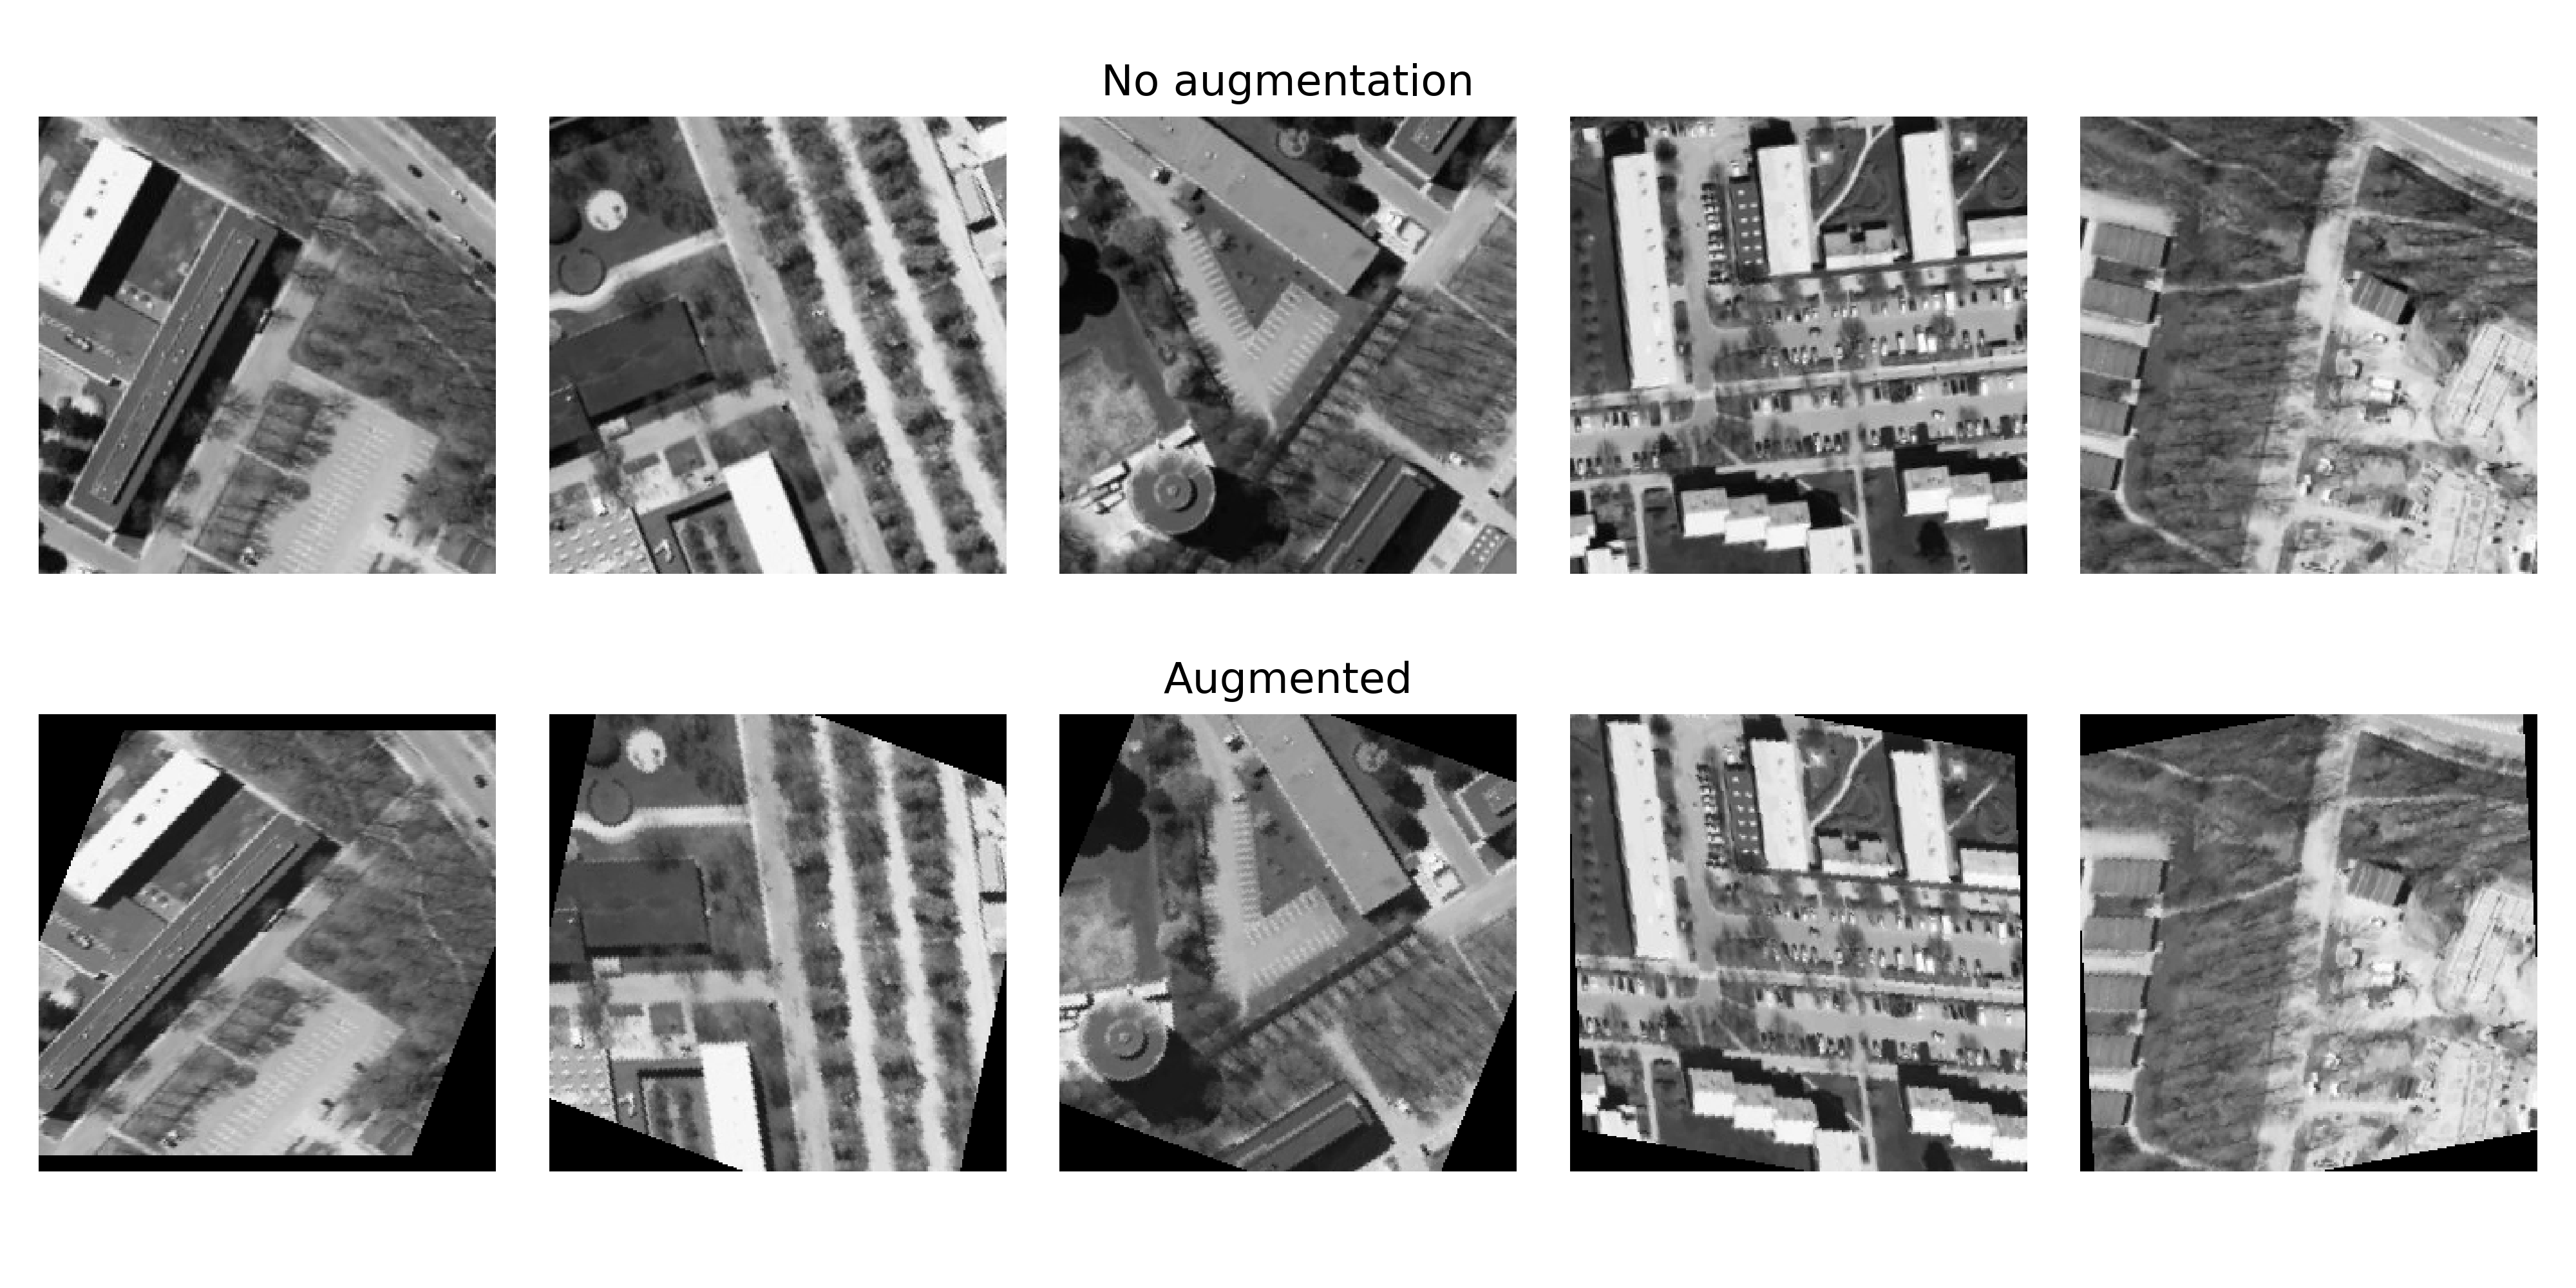
\includegraphics{chapters/part_pathloss/model_aided_paper/data_augmentation.png}
    \caption{A random affine transformation of satellite images used for data augmentation.}
    \label{fig:data_augmentation}
\end{figure}

A significant number of experiments were completed for scanning hyper-parameters. A complete list of hyper-parameters can be found in Table \ref{tab:cnn_structure}, \ref{tab:nn_structure} and \ref{tab:hyperparam_rest}. A total of $177$ experiments were conducted using different image strategies; the specific number of experiments can be observed in Table \ref{tab:experiments}. The scanning was done with a random search technique, meaning the hyper-parameters were sampled using a uniform distribution between ranges of interest \cite{Bergstra2012RandomOptimization}. A learning rate scheduler was applied with a patience parameter of $5$ epochs. Meaning, if no improvement in test error has been observed for at least five epochs, the learning rate is reduced with a factor of 10. This is also termed, \emph{reducing learning rate on plateu} and has been shown to improve the convergence of \glspl{nn} \cite{SmithSuper-Convergence:Rates}. The training is terminated when the learning rate reaches a value of $< 10^{-8}$.

\def\arraystretch{1.5}
\begin{table}[]
\begin{center}
\begin{tabular}{ll}
\multicolumn{2}{c}{\textbf{CNN}}                                                       \\
\multicolumn{1}{l|}{Input ch.}           & 1                                          \\ \hline
\multicolumn{1}{l|}{No. of convolutions} & [200, 100, 50, 25, 12, 1]                  \\ \hline
\multicolumn{1}{l|}{Activation}          & \emph{ReLU}                                       \\ \hline
\multicolumn{1}{l|}{Kernel size}         & [(5,5), (3,3), (3,3), (3,3), (2,2), (2,2)] \\ \hline
\multicolumn{1}{l|}{Max pooling}         & 2                                          \\ \hline
\multicolumn{1}{l|}{Padding}             & 2                                          \\ \hline
\multicolumn{1}{l|}{Stride}              & 1                                         
\end{tabular}
\end{center}
\caption{Architecture of the \gls{cnn} used for processing satellite images as detailed in Fig. \ref{fig:satellite_model_setup_v2}}\label{tab:cnn_structure}
\end{table}



\begin{table}
\subfloat[][]{
\begin{tabular}{ll}
\multicolumn{2}{c}{\textbf{NN}}                                                       \\
\multicolumn{1}{l|}{Layer size} & [200, 200]                  \\ \hline
\multicolumn{1}{l|}{Activation}          & \emph{ReLU}                                     
\end{tabular}
}
\subfloat[][]{
\begin{tabular}{ll}
\multicolumn{2}{c}{\textbf{NN2}}                                                       \\
\multicolumn{1}{l|}{Layer size} & [200, 16, 1]                  \\ \hline
\multicolumn{1}{l|}{Activation}          & \emph{ReLU}                                     
\end{tabular}
}
\vspace{1em}
\caption{Architecture of the sub-models considered in the final model architecture. }\label{tab:nn_structure}
\end{table}

\begin{margintable}
\begin{tabular}{@{}ll@{}}
\toprule
\textbf{Parameter} & \textbf{Value}   \\ \midrule
Batch size         & $30$             \\
Epochs             & $100$            \\
Image Size         & $256 \times 256$ \\
Learning Rate      & $0.001$            \\
Augmentation Angle & $\pm 20^{\circ}$ \\
Weight Decay       & $0.0029$         \\ \bottomrule
\end{tabular}
\caption{Best performing hyper-parameters for model \emph{v2}}\label{tab:hyperparam_rest}
\end{margintable}


\begin{table}[]
\centering
\begin{tabular}{@{}ll@{}}
\toprule
\textbf{Images} & \textbf{Experiments} \\ \midrule
Gray-scale images            & 114                  \\
Color images                 & 48                   \\
No data augmentation         & 15                   \\ \midrule
\textbf{Total}               & \textbf{177}         \\ \bottomrule
\end{tabular}
\caption{Number of experiments conducted for different image strategies.}\label{tab:experiments}
\end{table}


\subsection{Results}

The performance of the hyper-parameters weight decay and the augmentation angle is observed in Fig. \ref{fig:hyperparameters_weight_decay} (lower is better). A trend in an increase in performance is observed for both test and training, for decreasing values of weight decay. The trend for the augmentation angle is not as clear, as shown by the standard deviation and the mean of the experiments. Even though the mean observed performance of $10^{\circ}$ is better than the mean performance of $20^{\circ}$, the $\sigma$ at $20^{\circ}$ brings the overall test error closer to the training error. Thus the best performing model was found among the models trained at $20^{\circ}$ of data augmentation angle. The best performing found hyper-parameters can be seen in Table \ref{tab:hyperparam_rest}.

\begin{figure}
    \centering
    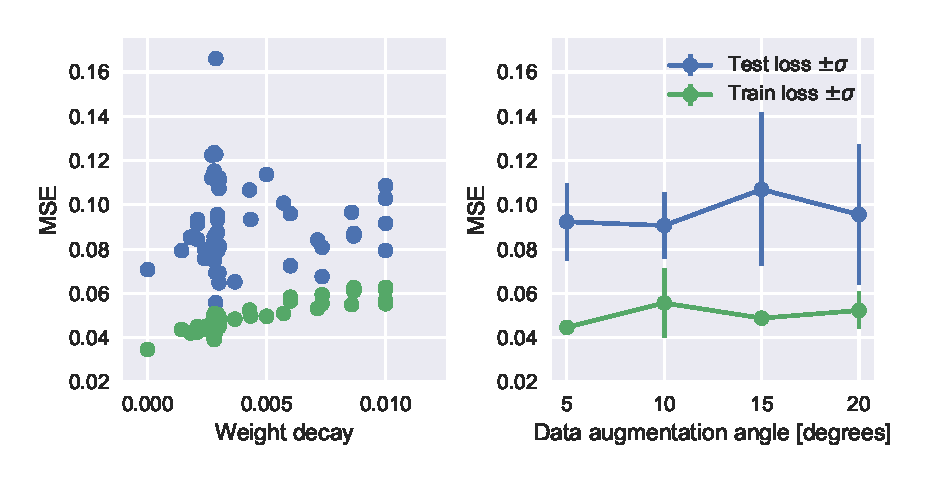
\includegraphics{chapters/part_pathloss/model_aided_paper/hyperparameters_grayscale.eps}
    \caption{Training and test error in MSE for weight decay and the augmentation angle.}
    \label{fig:hyperparameters_weight_decay}
\end{figure}


Using the traditional approaches of channel modelling, we can compare the performance. The comparison can be seen in terms of \gls{rmse} (lower is better) in Fig. \ref{fig:model_comparison_bar_group} for 811 and 2630 MHz respectively for the \uma{B} model and the ray-tracing model. The proposed approach is observed to outperform traditional modelling techniques for both 811 MHz and 2630 MHz, respectively. A gain of $\approx 1$ dB for 811 MHz, and $\approx 4.7$ dB for 2630 MHz is achieved compared to the traditional option, \uma{B}. 


\begin{figure}
    \centering
    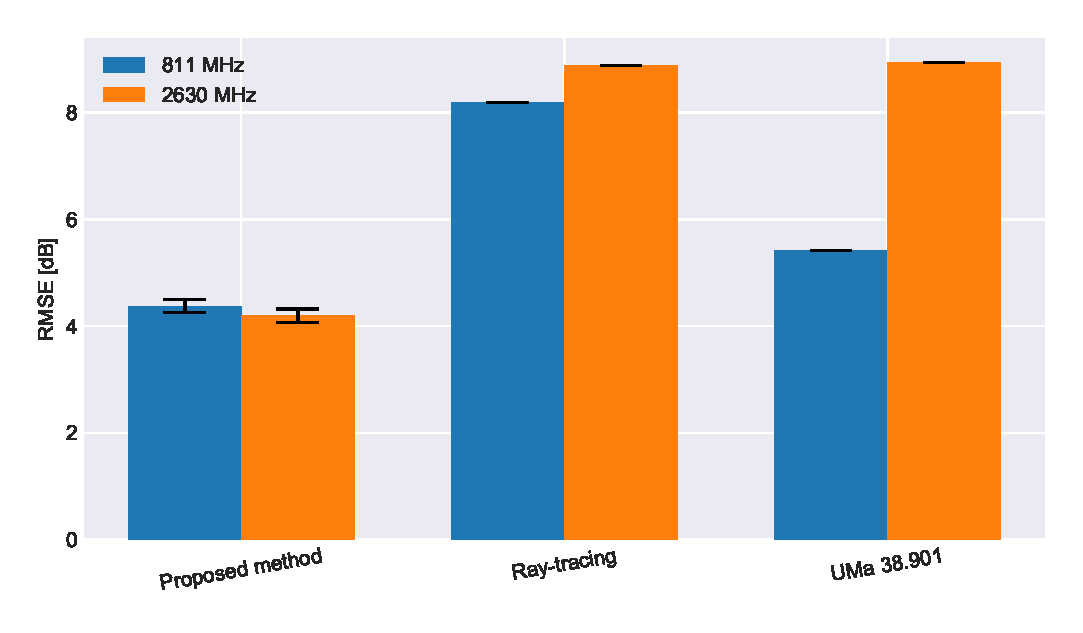
\includegraphics{chapters/part_pathloss/model_aided_paper/model_comparison_bar_group_std_split.eps}
    \caption{RMSE performance at 811 MHz and 2630 MHz for the proposed model \emph{v2} compared to traditional modelling techniques.}
    \label{fig:model_comparison_bar_group}
\end{figure}

The performance of the model is investigated in Fig. \ref{fig:train_models_barplot} where different versions of the proposed model are compared. More specifically, 1) no inclusion of a simple path loss (e.g. only data-driven), 2) no use of images (e.g. only features) and 3) with the aid from a simple path loss model and images (e.g. the complete proposed model). The \gls{rmse} in predictive performance, by including and processing satellite images, is  $\approx 4.37$ dB and $\approx 4.19 $ dB for $811$ and $2630$ MHz respectively. Meanwhile only using the features and being completely data-driven (e.g. no images or convolutional neural network and not aided by the path loss model) offer a performance of $\approx 5.12$ and $\approx 4.9$ dB for $811$ MHz and $2630$ MHz respectively. 

The introduction of the simple path loss model improves 1) the standard deviation of the predictive error and 2) the predictive performance. The standard deviation of the predictive error is the result of training multiple models with the same hyper-parameters, although instantiated with random weights. It can be seen as the error bars in Fig. \ref{fig:train_models_barplot}. By aiding the training process with a simple path loss model, the standard deviation of predictive performance was reduced from $\approx 0.57$ to $\approx 0.05$ dB. The performance increase can be observed to be $\approx 0.19$ and $\approx 0.54$ dB for 811 and 2630 MHz respectively comparing the fully data-driven approach and the introduction of a simple path loss model. 

The observed performance of the complete model (thus the use of satellite images and aided by a path loss model) increases the predictive performance, however with a slight increase in the standard deviation of prediction. More specifically, the gain provided by including images (compared to only using features) can be observed to be $\approx 0.55$ and $\approx 0.15$ for $811$ and $2630$ MHz respectively. The standard deviation increased to $\approx 0.05$ to $\approx 0.12$ dB. 

In summary, aiding the model with a path loss model improved the predictive capability by $\approx 0.54$ dB at $2630$ MHz while a reduced improvement was seen at $811$ MHz of $\approx 0.19$ dB. Including the images improved performance additionally by $\approx 0.55$ dB at $811$ MHz and $\approx 0.15$ dB at $2630$ MHz.

\begin{figure}
    \centering
    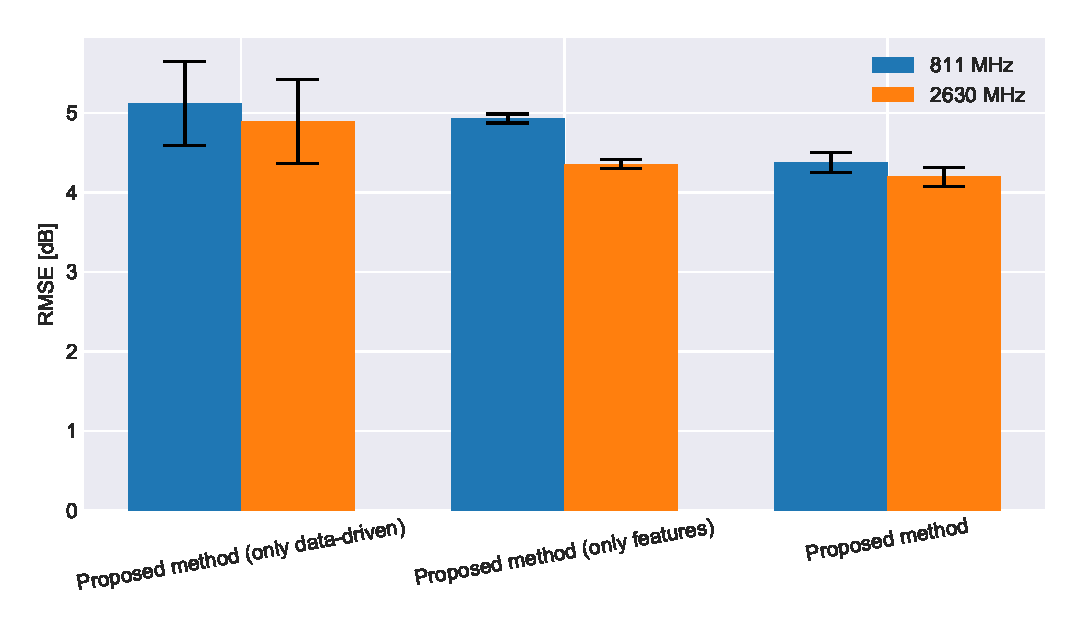
\includegraphics{chapters/part_pathloss/model_aided_paper/trainedmodels_barplot.eps}
    \caption{Comparison of different model techniques and structures.}
    \label{fig:train_models_barplot}
\end{figure}

The result of applying data augmentation can be observed in Fig. \ref{fig:dataaugmentation_training_test_error}. The test set is evaluated for each training epoch, thus providing the test and training error with and without data augmentation. A significant reducing in the generalization gap is observed and reduced from $\sim 0.13$ to $< 0.09$. 

\begin{figure}
    \centering
    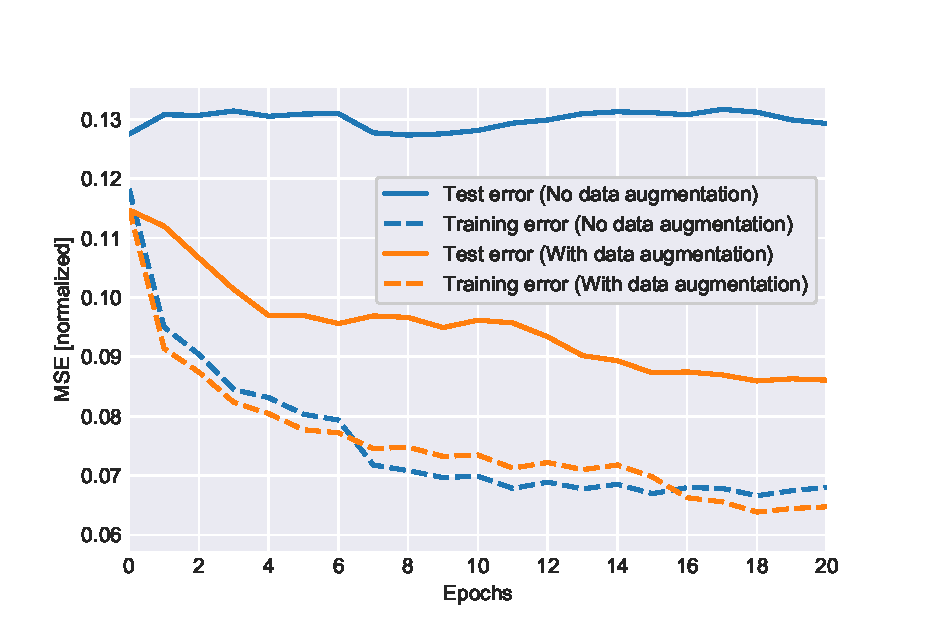
\includegraphics{chapters/part_pathloss/model_aided_paper/dataaugmentation_training_test_error.eps}
    \caption{The test and training error evaluated with and without the use of data augmentation techniques.}
    \label{fig:dataaugmentation_training_test_error}
\end{figure}

The output of $z(\cdot)$ as noted by Eq. (\ref{eq:model}) can be observed in Fig. \ref{fig:rsrp_correction_hist} for both 811 and 2630 MHz. The Deep Learning model produces thus a correction-element to the simple link budget estimation. The correction is similar to a Gaussian distribution, which is the model prerequisite and also how large-scale fading can be modelled. It should be noted that the distributions are not entirely centred, which illustrates a calibration offset. No gain was observed in re-calibrating the model such the mean was centred around $0$, e.g. $\mathcal{N}(0, \sigma)$.

\begin{figure}
    \centering
    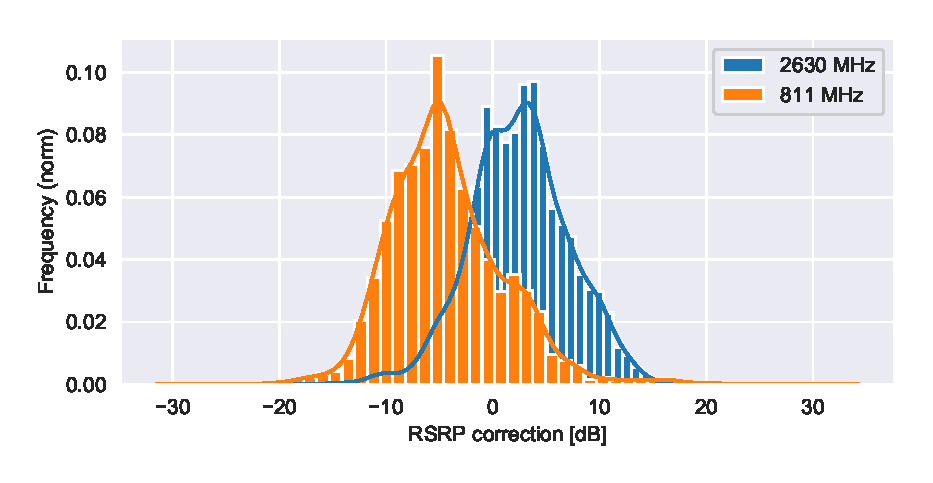
\includegraphics{chapters/part_pathloss/model_aided_paper/rsrp_correction_hist.eps}
    \caption{RSRP correction as noted by the output of $z(\cdot)$ in Eq. (\ref{eq:model}).}
    \label{fig:rsrp_correction_hist}
\end{figure}

The distributions of the \gls{rsrp} measurements and the prediction can be seen in Fig. \ref{fig:dist_pred_target} for both 811 and 2630 MHz. The performance difference between 811 and 2630 MHz, (as visualized by Fig. \ref{fig:model_comparison_bar_group}) comes to show here. A visually pleasing fit between predicted and measured is observed for 2630 MHz, while at 811 MHz, the model have issues with values of \gls{rsrp} around $-100$ to $-90$ dBm.

\begin{figure}
    \centering
    \subfloat[811 MHz]{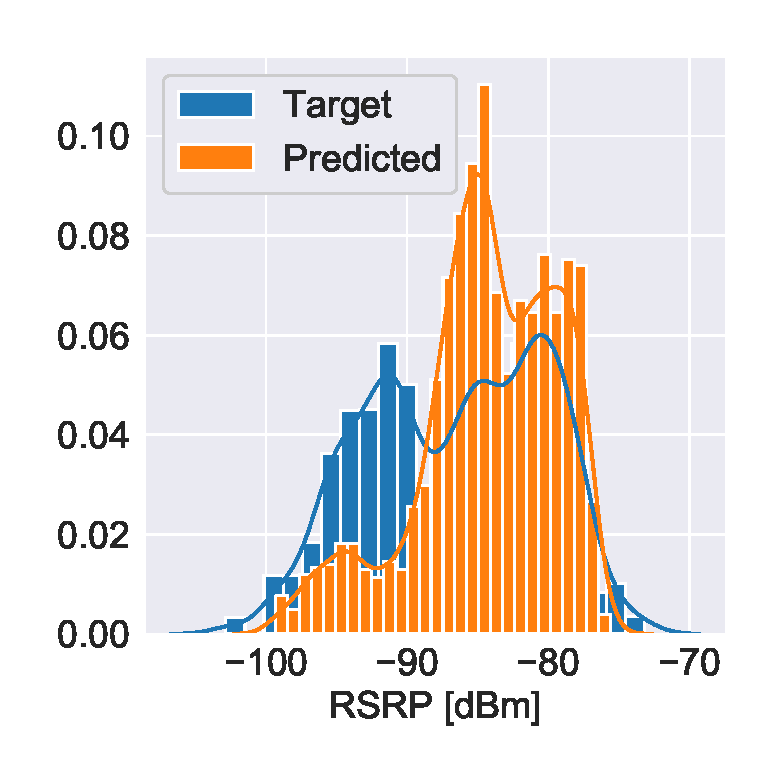
\includegraphics[width=0.4\textwidth]{chapters/part_pathloss/model_aided_paper/hist_63b17fa0-89e0-440b-952c-aa7f2e63e49c_811mhz.eps}\label{fig:dist_811}}  
    \subfloat[2630 MHz]{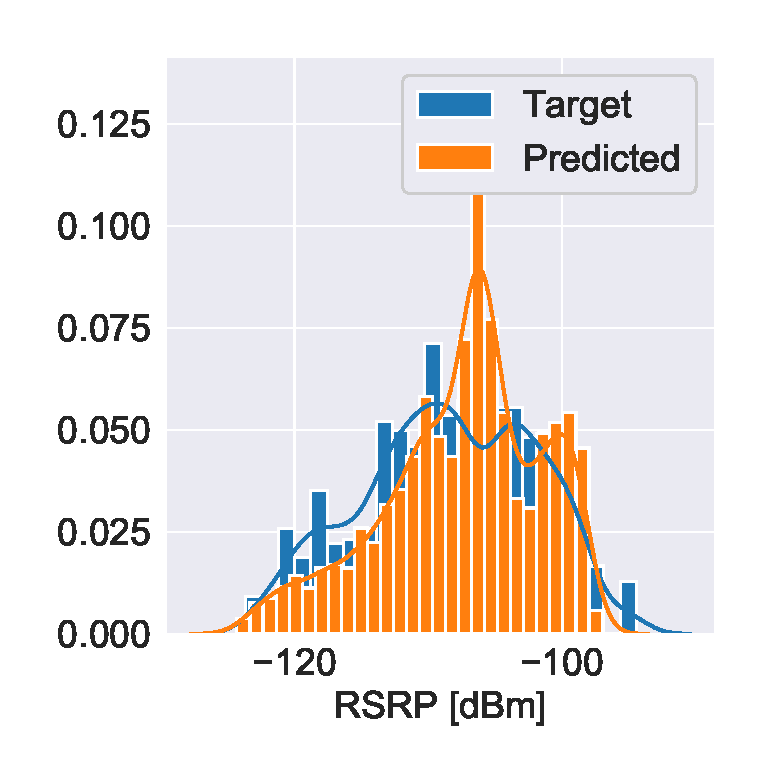
\includegraphics[width=0.4\textwidth]{chapters/part_pathloss/model_aided_paper/hist_63b17fa0-89e0-440b-952c-aa7f2e63e49c_2630mhz.eps}\label{fig:dist_2630}}
    \caption{Distribution of RSRP for 811 (a) and 2630 (b) MHz on the test set and the model output.}
    \label{fig:dist_pred_target}
\end{figure}

\subsection{Discussion}
The proposed approach is capable of outperforming traditional methods such as ray-tracing and empirical models. The predictive performance improvement at $2630$ MHz is $\approx 4.7$ dB while $\approx 1$ dB of gain is achieved at 811 MHz. The performance at 2630 MHz indicates the necessity of data describing local variability, which is not present in either the implemented ray-tracing model (limited clutter detail) or the empirical model. Clutter data is, however, observable in the proposed satellite images. The result indicates that this is not solely caused by including satellite images. The specific performance gain offered by the inclusion of the images is documented to be, on average, $\approx 0.8$ dB. Thus, the performance increase (compared to the traditional methodologies) seem to overall indicate the usefulness of \gls{nn} in path loss predictions. The majority of the performance increase is not caused by the inclusion of satellite images but rather the adaptive nature of \gls{nn}. However, by including the images and aiding the model with a simple path loss model, additional improvements to performance are achieved. 

The area spanned by the image offer details of clutter, nearby buildings and even parked cars. However, the area spanned by the images might contain details not relevant to differences in frequency. For instance, higher attenuation is associated with higher frequencies when it comes to clutter data due to the lower wavelength. In this case, it might be more relevant to include a more detailed version of the image spanning a reduced area. Moreover, it might be that the images simply contain too much information necessary for relevant propagation statistics. Such insight was gained during the hyper-parameter scanning, of which many experiments were conducted. Likely, simplistic images or the vectorization of such images (e.g. footprints/outlines of buildings) may improve the predictive performance, or in any case, enhance the task of finding the best-performing hyper-parameters.

The task of hyper-parameter scanning is complex and time-consuming. From the results, it is clear that performance improvements have been achieved in both utilizing features, a simple path loss model and satellite images. However, it should be noted that the documented hyper-parameters is an attempt at an optimum solution. It is likely that better hyper-parameters can be found using extensive scanning and possibly even Machine Learning-based sampling methodologies as documented in Chapter \ref{ch:mlbasics}. The model achieved requires approximately 300 experiments, each with 240 minutes of training time. The amount of experiments completed leads to the discussion of complexity. It is argued that the proposed method requires reduced complexity as compared to a traditional ray-tracing approach. The geostatistics and data necessary for local variability approximations are embedded into the supplied images and requires only the convolution and multiplication operations for extracting the \emph{correction} to a predicted path loss. It can be argued that the model only needs to be trained once, upon discovery of the best hyper-parameters. So in short, the complexity of the trained method solely lies in the prediction time and the memory necessary hereof. 

\subsection{Conclusion}\label{subsec:conclusion_v2}
The introduction of a simple path loss model (expert knowledge) for aiding the training process, in combination with satellite images, have improved the overall generalization properties of the Deep Learning model. The study items identified in \emph{version 1} have successfully been explored in an attempt to quantify the properties of the proposed approach and achieve insight into the specific prediction improvements by including satellite images. Furthermore, compare how the method performs to traditional approaches. The technique is capable of improving prediction accuracy by $\approx 1$ dB at $811$ MHz and $4.7$ dB at $2630$ MHz. The model provides an average prediction error of $\approx 4.1$ dB when predicting \gls{rsrp} in an unseen area for both $811$ and $2630$ MHz, which is a significant improvement to traditional methodologies. It is furthermore concluded that the complexity of the model is primarily associated with the untrained model, e.g. hyper-parameters and the selection hereof. The trained model is capable, with only position and available satellite images to produce an accurate prediction of receiver power in unseen areas.


\section{Reduced image complexity (v3)}\label{sec:osm_v3}
The implication of utilizing both satellite images and expert knowledge (in terms of a path loss model) requires further investigation and explorations. In particular, it is of interest to effectively reduce the model complexity to enable a more transparent inference of the prediction capability. Additionally, and possibly, more importantly, it is of great interest to validate the approach by using inherently different data sources. 

In the work \cite{Thrane2020DeepKnowledge}, the proposed approach is validated using simplified geographical images and additional drive test data. More specifically, this includes the use of so-called \emph{OpenStreetMap} data to supply the needed information for the used images. Furthermore, to enable generalization and interpolation between inherently different data sources, some changes were conducted to the features. The approach of this is visualized in Fig. \ref{fig:version3_architecture_figure}.

\begin{figure*}
    \centering
    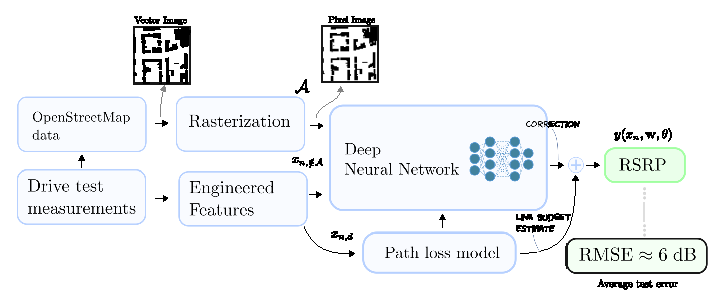
\includegraphics{chapters/part_pathloss/osm_images_paper/figures/version3_architecture_figure.eps}
    \caption{Architecture is set to utilize images provided by \gls{osm} instead of satellite images.}
    \label{fig:version3_architecture_figure}
\end{figure*}




\subsection{German measurements}

The experimental measurements of the previously used drive test data (See appendix \ref{app:drive_test_study_2017}, \cite{1xf4-eg98-19}) is appended with data from Dortmund, Germany \cite{SliwaEmpiricalNetworks}. The dataset contains measurements from multiple \glspl{mno} in different propagation scenarios at different operating frequencies. The essential characteristics can be seen in Table \ref{tab:drive_test_data_total}. The fundamental characteristics of the data allow for engineering the relevant features required for applying the proposed \gls{dl} model.

\begin{table*}[h]
\footnotesize
\begin{tabular}{@{}llll@{}}
\toprule
Dataset      & Samples & MNOs & Frequencies  [MHz]       \\ \midrule
DK Campus    & $57586$   & $1$    & $[811, 2630]$ \\
GER Campus   & $8579$    & $3$    & $[850, 860, 1815, 1845, 1865, 2630]$                   \\
GER Urban    & $11921$   & $3$    &  $[850, 860, 1845, 1865, 2630, 2650, 2680]$ \\
GER Suburban & $27152$   & $3$    &  $[850, 860, 1815, 1845, 1865,2630]$                   \\
GER Highway  & $20662$   & $3$    & $[850, 860, 870, 950, 1815, 1845, 1865,2630]$                    \\ \midrule
Total        & $125900$  &      &                     \\ \bottomrule
\end{tabular}
\vspace{1em}
\caption{Additional drive test data is available for training and testing consisting of various transmission frequencies.}\label{tab:drive_test_data_total}
\end{table*}

\subsection{Methodology}\label{subsec:osm_methodology}

Upon initial prototyping of the proposed method, it was found that the general features of \gls{gnss} positions, e.g. latitude and longitude coordinates caused severe extrapolation issues. More specifically, the model attempted to interpolate between the coordinates. The importance of the coordinates to the prediction of \gls{rsrp} caused the model to learn latent features of spatial importance. When evaluating the methodology in a different region (significant difference in latitude and longitude coordinates), the trained model would then provide a wrong interpretation of the spatial features by interpolating between coordinates. For this reason, a few changes to the formalized of the required engineered features were made. More specifically this resulted in

\begin{equation}
    x_n = [v, d, \Delta_\text{lat}, \Delta_\text{lon},  f_c, \mathcal{A}]
\end{equation}

Where $v$ is the velocity of the vehicle, $d$ is the distance in $3$D, $\Delta_\text{lat}$, $\Delta_\text{lon}$ are the difference in latitude and longitude between the receiver and the \gls{enb} respectively. $f_c$ is the carrier frequency in MHz, and $\mathcal{A}$ is the new simplified image.

The image was constructed similarly as \emph{v1} and \emph{v2}, using a \gls{roi} and a rotation towards the transmitter. Instead of the rotation causing the transmitter to be direction south (down) in the image, the image was rotated such that a direct path is to the east (right) in the image. Any performance gains did not cause this change, but rather ease of implementation. An example of such an image can be seen in Fig. \ref{fig:roi_image_preperation}. The area spanned by the image was adjusted to find the optimum use of the images. The rasterized image was kept constant at a size of $64 \times 64$ pixels. The images were extracted with the tool as documented in \cite{SliwaLightweightNetworks}. Data augmentation, as discussed in Section \ref{sec:training_v2}, was applied similarly.


\begin{figure}
    \centering
    
\includegraphics{chapters/part_pathloss/osm_images_paper/figures/map_to_image.eps}
    \caption{The \gls{roi} was determined around the measurement position spanning a variable size of area covered.}
    \label{fig:roi_image_preperation}
\end{figure}

\subsection{Model architecture}

The model architecture was kept similar to the one used in \emph{v2} embedding expert knowledge of path loss. A change to model complexity was necessary due to the simplification of 1) the engineered features and 2) the geographical images. The general idea of the model architecture is identical to that of Fig. \ref{fig:combined_model_approach} and Fig. \ref{fig:satellite_model_setup_v2}. The reduction in model complexity resulted in a significant increase in the number of hyper-parameters scanned and the automatization hereof. A Bayesian optimization scheme was applied to find the most probable hyper-parameters given the weight space provided by the final test error \cite{YuHyper-ParameterApplications, wandb}. Over $500$ experiments of different hyper-parameters and combinations hereof was conducted, resulting in a large model complexity reduction. An example of the hyper-parameter experiments can be found in Fig. \ref{fig:hyper-paramters_scan}. The final achieved hyper-parameters can be found in Table \ref{tab:hyper-parameters}.

Specifically, a reduction of convolutional filters can be observed. For instance, the first layer of the \gls{cnn} is reduced with $\approx 170$ filters compared to \emph{v2}. Furthermore, the size of the fully-connected layers processing the engineered features has also seen a reduction from $200$ to $32$. Additionally, the last \gls{nn} sub-module has been reduced from $200$ to $16$. This reduction has reduced not only the memory footprint of the proposed model but also the training performance and thus the resulting inference performance. Specifically, the model complexity reduction has resulted in sub-millisecond prediction times (accelerated with a GPU). 

\begin{figure*}
    \centering
    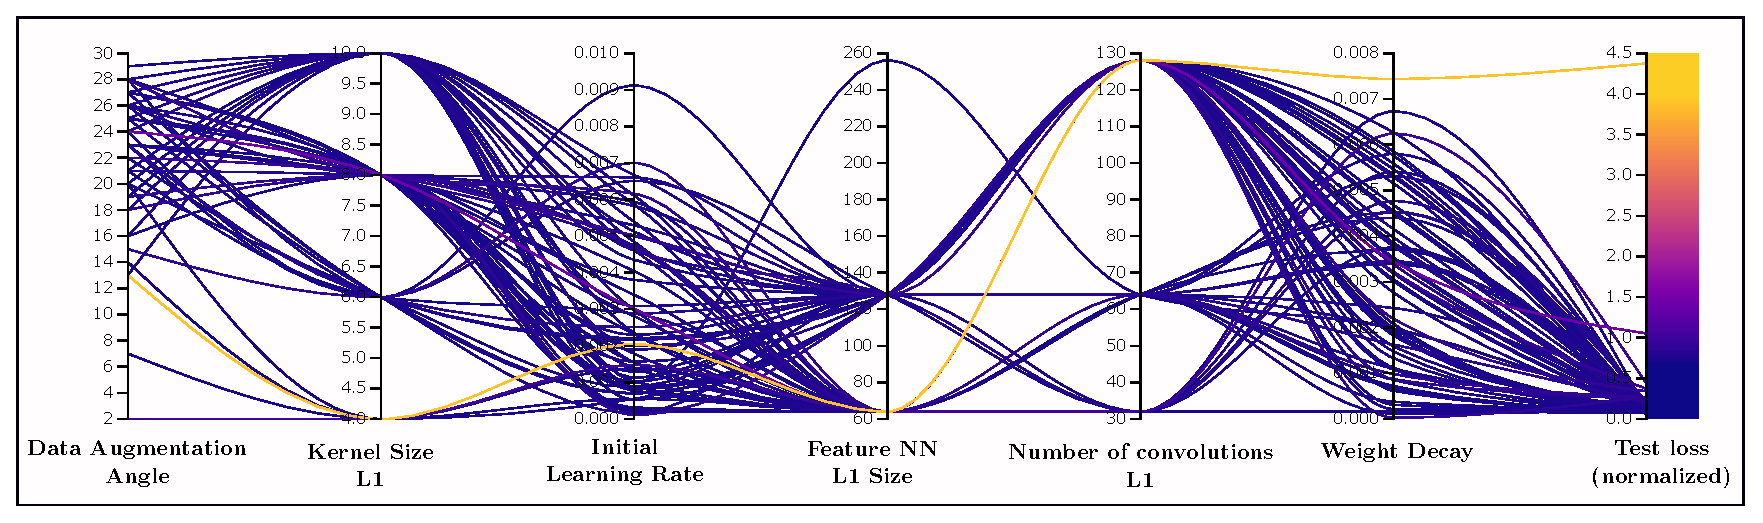
\includegraphics{chapters/part_pathloss/osm_images_paper/figures/hyperparameter_scan.eps}
    \caption{Bayesian optimization applied during hyper-parameter scan \cite{wandb}.}
    \label{fig:hyper-paramters_scan}
\end{figure*}


\begin{table}[]
    \centering
    \footnotesize
    \caption{Hyper-parameters for the deep neural network model.}\label{tab:hyper-parameters}
    \begin{tabular}{@{}lll@{}}
    \toprule
    \textbf{Parameter}          & \textbf{Value}                &  \\ \midrule
    Weight decay                & 8e-4                          &  \\
    Learning rate               & 1e-3                          &  \\
    Filters                     & [32, 32, 10, 1]               &  \\
    Kernel size                 & [(5,5), (3,3), (3,3), (2,2)]  &  \\
    Max pooling                 & [2, 2, 2, 2]                  &  \\
    Feature NN layer size       & [32, 32]                      &  \\
    Output NN layer size        & [16, 16]                      & \\
    Image augmentation angle    & 20                            & \\
    Image size                  & $64~\text{px} \times 64~\text{px}$                & \\
    Batch size                  & 12                            &  \\ \bottomrule
\end{tabular}
\end{table}

\newpage
\newpage


\subsection{Comparative results}
The results of utilizing simple geographical images instead of the satellite images can be seen in Fig. \ref{fig:model_comparison_access}. The overall performance can be seen to be identical to that of \emph{v2} on the same test set. A slight decrease at 811 MHz in performance is observed, however with a slight difference in the standard deviation across several version of the final trained models. Similar performance at $2630$ MHz was achieved.

\begin{figure}[h]
    \centering
    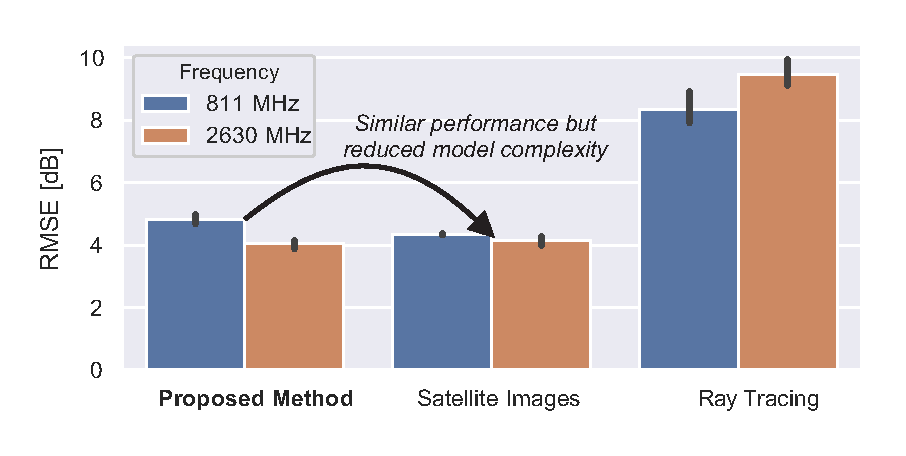
\includegraphics{chapters/part_pathloss/osm_images_paper/figures/model_comparison_access.eps}
    \caption{Comparison of simple \gls{osm} images with satellite images and ray-tracing.}
    \label{fig:model_comparison_access}
\end{figure}


To further explore the performance across all of the data subsets, a cross-validation approach was employed. Specifically, this entailed training on the majority of subsets while keeping one scenario for testing, repeated for all subsets. For instance, when refereed to the performance of \texttt{GER Campus} - it is trained on all other subsets of data excluding the \texttt{GER Campus} subset. The generalization gap for all subsets can be seen in Fig. \ref{fig:generalization_gap}. The figure shows the difference between the test and training error for each training epoch; in other words, how well the trained model performs on the remaining subset. If close to zero a generalization across the data subset is achieved. It can be seen that the \texttt{GER Campus} subset achieves by far the best generalization performance. The worst generalization is achieved for the \texttt{DK campus} subset. Both the \texttt{GER suburban} and \texttt{GER urban} subset achieved similar performance.

\begin{figure}[h]
    \centering
    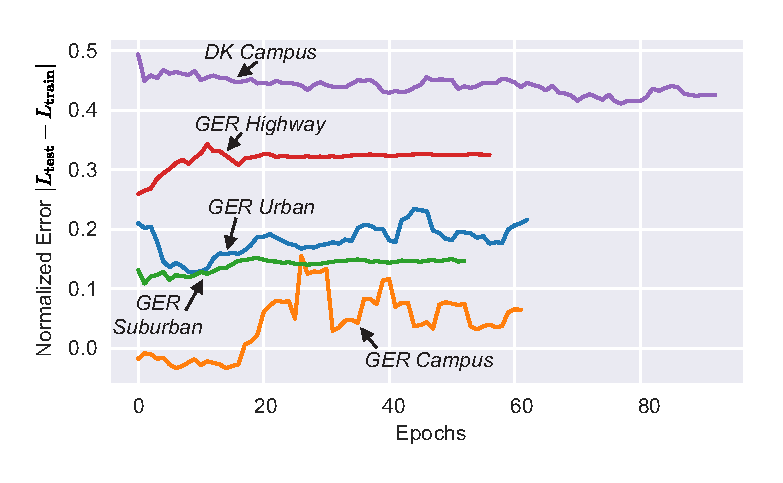
\includegraphics{chapters/part_pathloss/osm_images_paper/figures/training_test_error_crossvalidation_diff.eps}
    \caption{Generalization gap for all subsets.}
    \label{fig:generalization_gap}
\end{figure}

The performance is also evaluated in terms of \gls{rmse} (see \ref{eq:rmse}). This can be observed in Fig. \ref{fig:rmse_boxplot_osm} (lower is better). The cross-validated performance is shown for all subsets. The \gls{rmse} is computed for all mini-batches of samples, thus the figure shows the average \gls{rmse} across all mini-batches and the resulting standard deviation. Furthermore, outliers are also displayed. The best performance is achieved on the \texttt{GER campus} subset with a \gls{rmse} of $6.3$ dB and $\sigma = 3.6$ dB. The worst performance is seen on the \texttt{GER Highway} subset, with an \gls{rmse} of $9.7$ dB and $\sigma = 1.2$ dB.


\begin{figure}[h]
    \centering
    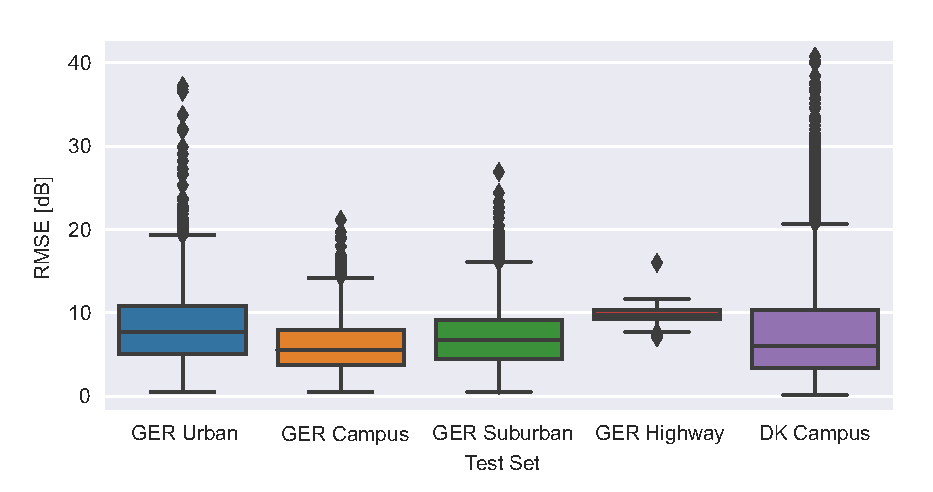
\includegraphics{chapters/part_pathloss/osm_images_paper/figures/RMSE_boxplot.eps}
    \caption{Cross-validation results of all data subsets. Each subset is evaluated using a model trained on the remainder of the subsets.}
    \label{fig:rmse_boxplot_osm}
\end{figure}

\subsection{Image distance results}
As a result of the reduced model complexity, additional exploration of the importance of spatial dependency has been completed. This has resulted in the comparison of so-called \emph{full-size} images instead of the \emph{regular} \gls{roi} images (centered around the measurement coordinate). The \emph{full-size} images consider not only the receiver location but also the transmitter location. In other words, both positions are within the spanned \emph{full-size} image. Thus, if the antenna separation distance increase, the area spanned by the image increase.  \emph{Regular} images have a constant area covered by the image regardless of antenna separation distance. A so-called \emph{violin} plot is found in Fig. \ref{fig:rmse_violin_image_comparison}. The figure shows the estimation of the kernel density provided by batch-wise \gls{rmse} computation. The distribution and range of using \emph{full-size} images are noticeably different than using the \emph{regular} images spanning 250 meters. More so, the number of outliers (and the range) increased. Using \emph{regular} images resulted in an \gls{rmse} of $6.3$ dB while an \gls{rmse} of $7.3$ dB was achieved using the \emph{full-size} images.



\begin{figure}[h]
    \centering
    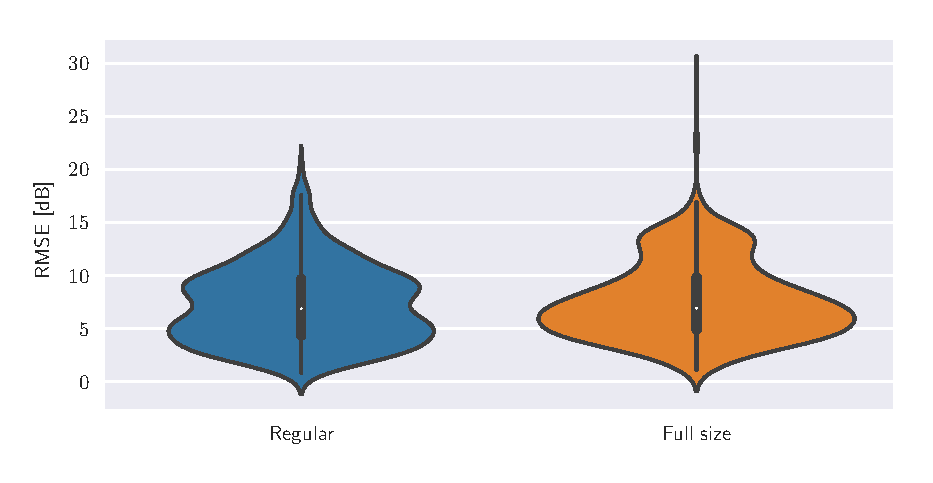
\includegraphics{chapters/part_pathloss/osm_images_paper/figures/RMSE_violin.eps}
    \caption{Performance comparison of varying the area spanned by the images. Evaluated on \texttt{GER Campus}, trained on the remainder.}
    \label{fig:rmse_violin_image_comparison}
\end{figure}


The impact of the area spanned by the \gls{roi} is evaluated in Fig. \ref{fig:boxplot_ci_image_distance}. The area spanned by the images are varied, while the pixel size of the image is kept constant. The performance is evaluated concerning the \texttt{GER Campus} subset, with a model trained on the remainder of the subsets. The best performing images were found spanning a distance of $250-300$ meters with similar predictive performance. Decreasing the distance spanned by the images offers a slight increase in \gls{rmse}. The same is observed for increasing the distance spanned by the images.

\begin{figure}
    \centering
    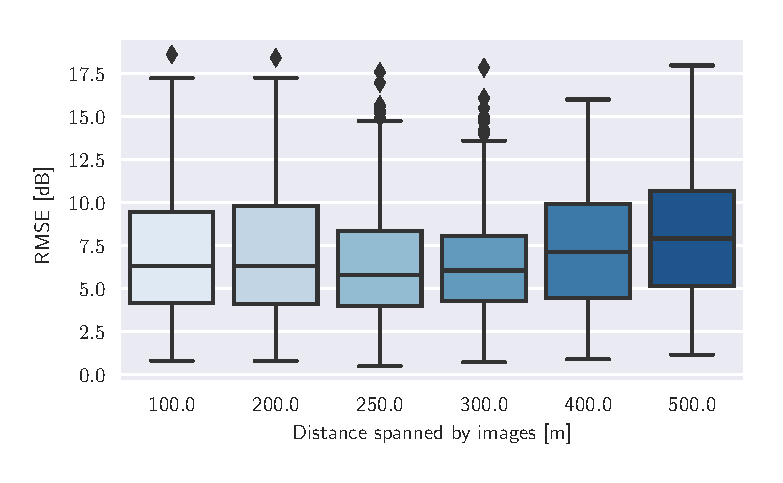
\includegraphics{chapters/part_pathloss/osm_images_paper/figures/boxplot_ci_image_distance.eps}
    \caption{Performance comparison of utilizing different distances for the images. The performance is with respect to the \texttt{GER Campus} subset, trained on the remainder.}
    \label{fig:boxplot_ci_image_distance}
\end{figure}

\subsection{Heatmap generation}

The trained models can effectively extrapolate and interpolate measurements in the area of the originated drive tests. An example of this for 2630 MHz can be seen in Fig. \ref{fig:osm_heatmap}. The model is trained on the entirety of the data points in the \texttt{DK Campus} subset. A grid of features is generated for all latitude and longitude coordinates in the area of interest. The model is then evaluated for the generated features. The results show a feasible range of predicted \gls{rsrp} values, in the range of $-80$ to $-140$ dBm. Furthermore, an increase in \gls{rsrp} is seen near the \gls{enb} location. 

\begin{figure}[!h]
    \centering
    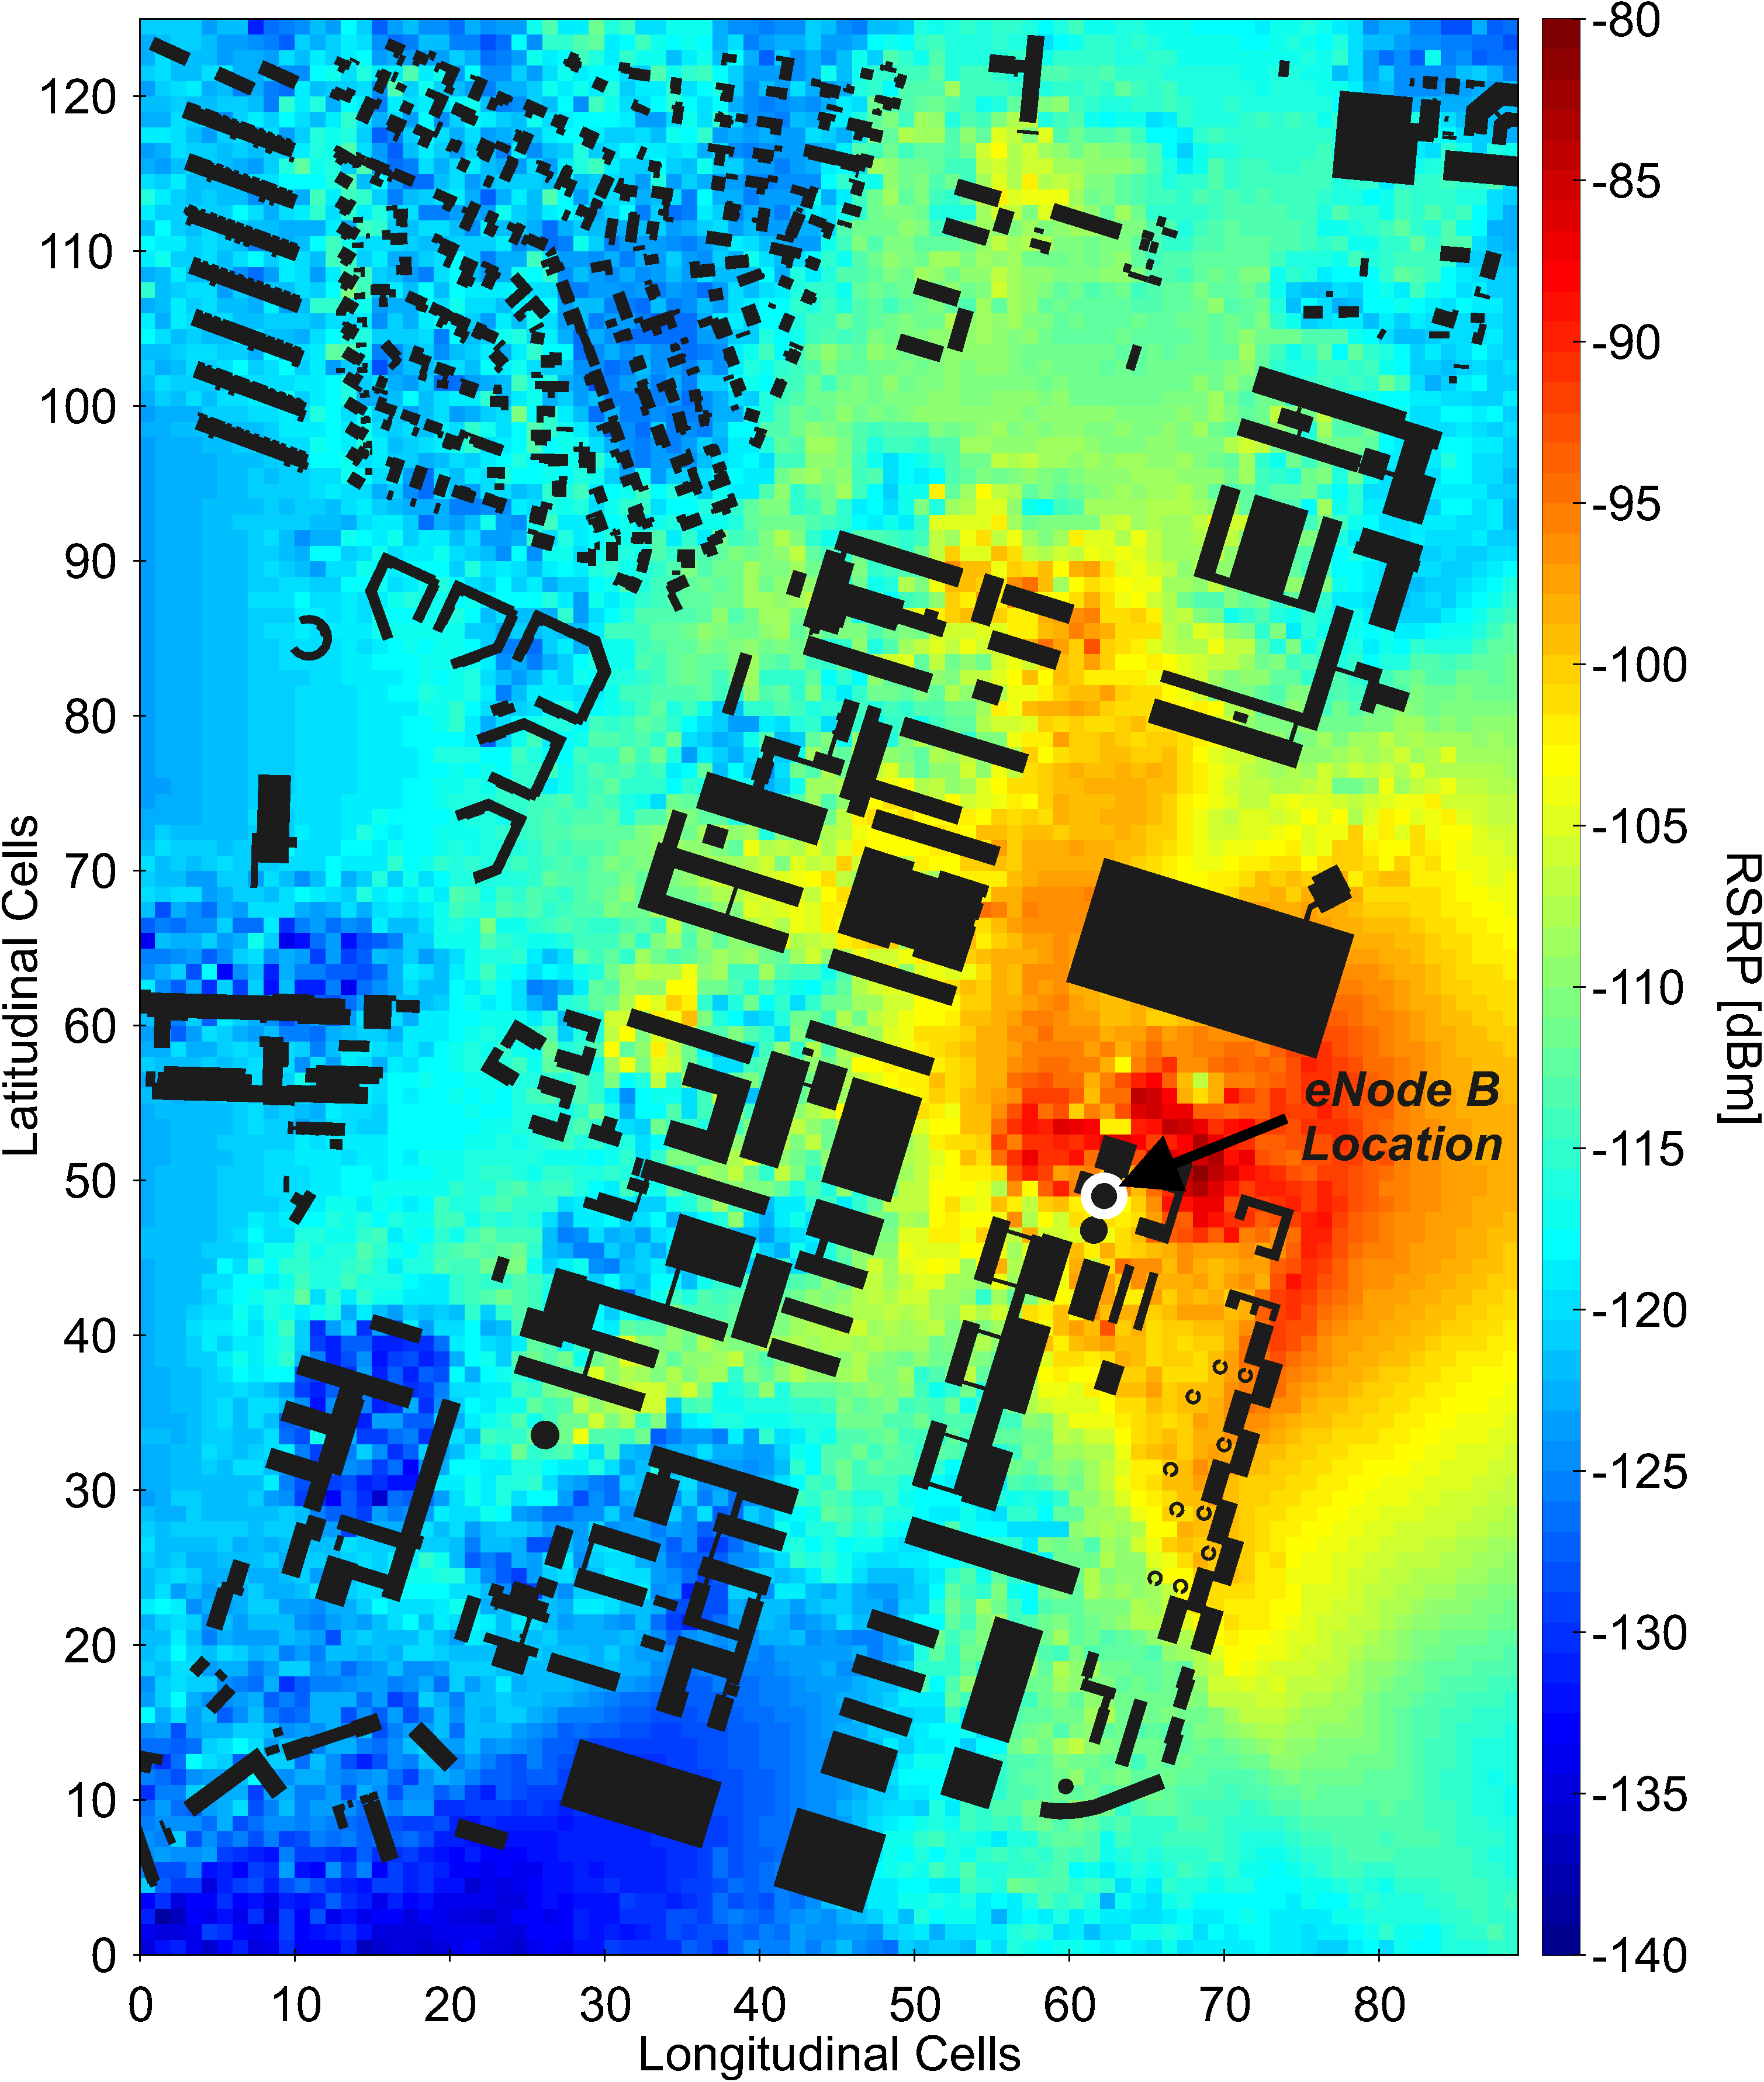
\includegraphics{chapters/part_pathloss/osm_images_paper/figures/heatmap.pdf}
    \caption{Extrapolated heatmap at 2630 MHz using generated features for all latitude and longitude coordinate pairs.}
    \label{fig:osm_heatmap}
\end{figure}

\subsection{Discussion}

A necessary procedure of the proposed method is experimental validation from inherently different data sources. The above-documented results contribute towards such a validation. The use of the German-based datasets is an essential first step in showing the properties and gains of the proposed method. The German-based datasets consist of several frequencies not present in the original \texttt{DK} dataset. More so, it effectively doubles the number of available samples for learning. The procedure for generating the geographical images is simplified as it only requires \gls{osm} data. 

The generalization performance has been analyzed using a cross-validation approach. A necessity of this approach is multiple trained models which is contingent on feasible training times. Evaluating the \texttt{DK Campus} subset is effectively extrapolation across data with an inherently different origin. The results indicate that the generalization across datasets with different data origin is possible and offer accurate performance $\text{\gls{rmse}} = 7.8$ dB. However, by including data from different origins the accuracy is effectively improve as is indicated by the performance $\text{\gls{rmse}} = 6.3$ dB of the \texttt{GER Campus} scenario. The  \texttt{GER Campus} is the campus of TU Dortmund, which does share many architectural similarities with the \texttt{DK Campus} scenario. The results indicate that this is inferred from data with a different origin. 

The geographical images supplied by a \gls{osm} pipeline have effectively resulted in a simplified training procedure and a significant reduction in hyper-parameters. Even with the reduction of hyper-parameters, the original reported gains (as seen in \emph{v2} and \cite{Thrane020ModelAidedDeepLearning}) on the \texttt{DK Campus} dataset are maintained. A direct result of this reduction is the main driver for the cross-validation procedure to be completed in a feasible time. The training time, with over double the amount of samples and a lower batch-size, is maintained at approximately $120$ minutes. The inference time is halved to sub-millisecond predictions.

The produced heatmap offers insight into the predictive capabilities of the method. Even though the heatmap is produced on the scenario at which it was trained, it still had to infer \gls{rsrp} for non-measured locations. The fact that the range of \gls{rsrp} values is within expected values is a favourable property of the trained \gls{nn}. Furthermore, the heatmap shows an increased intensity around the location of the \gls{enb}, which is probably. Finally, some sectorization of the \gls{enb} can, with some imagination, be observed. Future work of the methodology is not only to further test the generalization properties but also the performance to existing methods of producing radiomaps, for instance, compare the proposed approach to that of \emph{Kriging}.

% Altitude information embedding
Additionally, the images contain only information on the building footprints. It would be of great interest to study the embedding of altitude and height information into such images. 


\subsection{Conclusion}\label{subsec:conclusion_v3}
Simple geographical images, along with expert knowledge supply strong prior information for predicting \gls{rsrp} for unseen locations. It is shown that latent features for describing local radio characteristics can be found using simple geographical images. The proposed approach is vigorously validated on additional experimental data. The images were produced using a simplified pipeline utilizing \gls{osm} data and contain only information on buildings and the location. Images spanning a distance of $250-300$ meters was found to produce improved performance. The results show that the proposed method is able to generalize across inherently different data origins. The best predictive performance on an unseen propagation scenario is reported to be $\text{\gls{rmse}} = 6.3$ ($\sigma = 3.6$ dB) on a multitude of operating frequencies.





\section{Identified Challenges}\label{sec:identified_challenges_satellite}
A multitude of model architectures and training procedures have been documented throughout this Chapter. Along the way several pressing technical challenges have been identified. These can be reduced to the following items.

\begin{itemize}
    \item Convolutional layers are challenging to interpret.
    \item Embedding expert knowledge for other signal quality parameters.
    \item Clutter and Altitude/Height information not easily available.
\end{itemize}

The use of a \gls{cnn} for processing the images is a powerful tool for enabling latent features useful for signal quality parameter prediction. Essentially, \gls{cnn} use convolutional layers (or filterbanks) to apply a set of filters and feature extraction principles for reducing input images into useful features. In other words, the trained model consists thus of filters. The filters activate on important statistics present in the images, that are useful for the final predictors. Thus, in order to effectively improve the proposed methods, such filters needs to be further investigated and explored. However, such a testing and experimental procedure is not trivial and requires not only vigorous testing but also a significant number of samples for validating any resulting knowledge obtained. The addition of the German-based measurements enables such studies, therefor it is imperative for future studies that the learned filters are analysed.

It is shown that the model can be improved by embedding expert knowledge, in terms of a path loss model, into the training procedure. The results of the initial version (\emph{v1}) show that other signal quality parameters (such as \gls{rsrq} and \gls{sinr}) can be predicted with high accuracy. An identified challenge is the embedding of expert knowledge capable of aiding the prediction capabilities of such parameters. 

The use of simplified geographical images does not increase the prediction errors compared to utilizing high-resolution satellite images. In both cases no altitude or height information is embedded. Some height information are embedded in the satellite images, in terms of shadows of the resulting buildings and other details. However, as shown in state-of-the-art image segmentation algorithms, deducing building height from shadows alone is prone to significant errors. Thus, a challenge of the methodology would be to explore new avenues of embedding height information. In the \gls{osm} images, such a feature could be directly enabled onto building shapes by for instance using a color-mapping. Clutter data, important for higher frequencies (e.g. shorter wavelengths) is shown to have significant impact on the received power of the receiving devices. Thus being able to model such data is critical to accurate predictions. Therefor, extending the image information with clutter related data while keeping the data complexity low seems like a logical next step for the use of the methodology.


\section{Summary}\label{sec:satellite_image_discussion}
The process of utilizing satellite images for path loss prediction has been an ongoing process of relevant study items. The different iterative steps for improving and studying the approach has been documented throughout this chapter, an termed by the different \emph{versions}. The outcome of each iteration has extensively been discussed and can be summarized as follow:
\begin{itemize}
    \item \emph{Version 1} Initial exploration - Proof of concept. Generalization issues and further need for comparative studies.
    \item \emph{Version 2} Model-aided approach - Applied techniques for improving generalization and the comparison to traditional approaches.
    \item \emph{Version 3} Simplified images - Additional measurements from an inherently different origin. The study of simplistic images and the impact on predictive performance
\end{itemize}

\textcolor{red}{Maybe add figure here if time allows it}


The iterative improvements of the model has allowed for well-defined conclusions. Taking a step back, the knowledge obtained can be reduced for relevant terms associated with wireless communication and cellular networks. It was well known in literature that \gls{nn} can provide with highly accurate path loss predictions that can (possibly) assist in deployment and optimization processes of the cellular networks. However, what is not discussed is the underlying dangers of supervised learning. It can be seen throughout \emph{version 1} and also to some extent \emph{version 2} that high performance can be achieved on the dataset at which the model is trained. Which is obvious due to the fundamental principles of \gls{ml}. The dangers of supervised learning arise when the generalization is unexplored or with significant bias. This is explore and testing in \emph{version 3} by using a inherently different data source. If \gls{nn}-based path loss models are to be of any use, vigorous testing and comparative studies are essential otherwise such models are useless. The aim of the method developed throughout this PhD project has been to go beyond that and lay the foundation for methods that not only improve performance in terms of dB but also ensure the predictions are within reason and intuition. 

Much more data can essentially be integrated into path loss modelling using the principles documented throughout chapter. It is important that the complexity of such that (not only obtaining it but also processing it) remains low otherwise the models become useless for their sole purpose: \emph{To model capacity and coverage for the optimization of cellular systems and infrastructure.}